%  ==========================================================================
%  Single-file manuscript for Heritage (MDPI).  Everything -- layout, text,
%  tables and all seven figures (drawn natively with TikZ/pgfplots) -- is in
%  this one file.  Compile with pdfLaTeX (e.g. on Overleaf), running twice.
%
%  For the final submission, MDPI's official class can be used instead:
%  replace the block between "BEGIN MDPI-STYLE LAYOUT" and "END MDPI-STYLE
%  LAYOUT" by \documentclass[heritage,article,submit,pdftex,oneauthor]{Definitions/mdpi}
%  and keep the rest of the file unchanged.
%  ==========================================================================
%  ---------------- BEGIN MDPI-STYLE LAYOUT ----------------
\documentclass[10pt,a4paper]{article}
\makeatletter

\usepackage[T1]{fontenc}
\usepackage[utf8]{inputenc}
\usepackage{mathpazo}
\usepackage[scaled=0.86]{helvet}
\usepackage{microtype}
\usepackage{amsmath,amssymb,amsthm}
\usepackage{graphicx,xcolor,booktabs,array,tabularx,float,calc,ifthen}
\usepackage{changepage}
\usepackage{lineno}
\usepackage{fancyhdr,lastpage}
\usepackage[font={small},labelfont=bf,labelsep=period,justification=justified,singlelinecheck=false]{caption}
\usepackage[a4paper,left=5.6cm,right=1.9cm,top=2.4cm,bottom=2.4cm,headsep=0.8cm]{geometry}
\usepackage[hidelinks]{hyperref}
\newlength{\extralength}\setlength{\extralength}{3.7cm}
\definecolor{bluetext}{RGB}{0,78,145}
\newcommand{\firstpage}[1]{\gdef\@firstpage{#1}}
\newcommand{\pubvolume}[1]{}\newcommand{\issuenum}[1]{}\newcommand{\articlenumber}[1]{}
\newcommand{\pubyear}[1]{}\newcommand{\copyrightyear}[1]{}\newcommand{\externaleditor}[1]{}
\newcommand{\datereceived}[1]{}\newcommand{\daterevised}[1]{}\newcommand{\dateaccepted}[1]{}
\newcommand{\datepublished}[1]{}\newcommand{\hreflink}[1]{}
\newcommand{\TitleCitation}[1]{}\newcommand{\AuthorNames}[1]{}\newcommand{\AuthorCitation}[1]{}
\newcommand{\orcidA}{}\newcommand{\orcidB}{}
\newcommand{\Title}[1]{\gdef\@mdpititle{#1}}
\newcommand{\Author}[1]{\gdef\@mdpiauthor{#1}}
\newcommand{\address}[1]{\gdef\@mdpiaddress{#1}}
\newcommand{\corres}[1]{\gdef\@mdpicorres{#1}}
\renewcommand{\abstract}[1]{\gdef\@mdpiabstract{#1}}
\newcommand{\keyword}[1]{\gdef\@mdpikeyword{#1}}
\gdef\@mdpititle{}\gdef\@mdpiauthor{}\gdef\@mdpiaddress{}\gdef\@mdpicorres{}\gdef\@mdpiabstract{}\gdef\@mdpikeyword{}
\renewcommand{\familydefault}{\rmdefault}
\setlength{\parindent}{0.75cm}
\linespread{1.08}
\pagestyle{fancy}\fancyhf{}\renewcommand{\headrulewidth}{0pt}
\fancyhead[R]{\small\sffamily\@mdpijournal\ \the\year, \textit{x}, x \hfill \thepage\ of \pageref*{LastPage}}
\gdef\@mdpijournal{\textit{Heritage}}
\fancyheadoffset[L]{\extralength}
\fancypagestyle{plain}{\fancyhf{}\fancyhead[L]{\hspace*{0pt}\sffamily\large\bfseries\color{bluetext}Article}\fancyhead[R]{}\fancyheadoffset[L]{\extralength}}
\renewcommand{\section}{\@startsection{section}{1}{0pt}{12pt plus 2pt}{6pt}{\normalfont\normalsize\bfseries}}
\renewcommand{\subsection}{\@startsection{subsection}{2}{0pt}{9pt plus 2pt}{4pt}{\normalfont\normalsize\itshape}}
\renewcommand{\subsubsection}{\@startsection{subsubsection}{3}{0pt}{6pt}{3pt}{\normalfont\normalsize}}
\renewcommand{\thesection}{\arabic{section}}
\renewcommand{\@seccntformat}[1]{\csname the#1\endcsname.\ }
\AtBeginDocument{%
  \thispagestyle{plain}%
  \begin{adjustwidth}{-\extralength}{0cm}%
  {\raggedright\sffamily\bfseries\fontsize{18}{22}\selectfont\@mdpititle\par}\vspace{10pt}%
  {\raggedright\sffamily\bfseries\normalsize\@mdpiauthor\par}\vspace{6pt}%
  \end{adjustwidth}%
  {\footnotesize\@mdpiaddress\par\@mdpicorres\par}\vspace{8pt}%
  {\small\noindent\textbf{Abstract:} \@mdpiabstract\par\vspace{4pt}\noindent\textbf{Keywords:} \@mdpikeyword\par}%
  \vspace{4pt}\noindent\rule{\textwidth}{0.4pt}\vspace{2pt}%
  \linenumbers}
\newcommand{\backmatterhead}[1]{\par\vspace{4pt}\noindent\textbf{#1}\ }
\newcommand{\supplementary}[1]{{\small\backmatterhead{Supplementary Materials:}#1\par}}
\newcommand{\authorcontributions}[1]{{\small\backmatterhead{Author Contributions:}#1\par}}
\newcommand{\funding}[1]{{\small\backmatterhead{Funding:}#1\par}}
\newcommand{\institutionalreview}[1]{{\small\backmatterhead{Institutional Review Board Statement:}#1\par}}
\newcommand{\informedconsent}[1]{{\small\backmatterhead{Informed Consent Statement:}#1\par}}
\newcommand{\dataavailability}[1]{{\small\backmatterhead{Data Availability Statement:}#1\par}}
\newcommand{\acknowledgments}[1]{{\small\backmatterhead{Acknowledgments:}#1\par}}
\newcommand{\conflictsofinterest}[1]{{\small\backmatterhead{Conflicts of Interest:}#1\par}}
\newcommand{\abbreviations}[2]{{\small\backmatterhead{#1}\par\noindent #2\par}}
\newcommand{\reftitle}[1]{\section*{#1}}
\newcommand{\PublishersNote}[1]{}
\newcommand{\appendixtitles}[1]{}
\newcommand{\appendixstart}{\appendix\renewcommand{\thesection}{\Alph{section}}}
\renewenvironment{thebibliography}[1]{\nolinenumbers\small\list{\arabic{enumiv}.}{\settowidth\labelwidth{999.}\leftmargin\labelwidth\advance\leftmargin\labelsep\usecounter{enumiv}\itemsep 0pt}\sloppy}{\endlist}
\def\@cite#1#2{[{#1\if@tempswa , #2\fi}]}
\makeatother
%  ---------------- END MDPI-STYLE LAYOUT ----------------
%=================================================================
% MDPI internal commands -- do not modify
\firstpage{1}
\makeatletter
\setcounter{page}{\@firstpage}
\makeatother
\pubvolume{1}
\issuenum{1}
\articlenumber{0}
\pubyear{2026}
\copyrightyear{2026}
\datereceived{ }
\daterevised{ }
\dateaccepted{ }
\datepublished{ }
\hreflink{https://doi.org/}

%=================================================================
% Additional packages and author macros
\usepackage{multirow}
\usepackage{sansmath}
\usepackage{tikz}
\usetikzlibrary{arrows.meta,calc}
\usepackage{pgfplots}
\pgfplotsset{compat=1.16}
\usepgfplotslibrary{groupplots}
\definecolor{cteal}{HTML}{2F5D62}\definecolor{cred}{HTML}{A44A3F}\definecolor{cochre}{HTML}{B08A45}
\definecolor{cgray}{HTML}{666360}\definecolor{clgray}{HTML}{9A9791}\definecolor{csage}{HTML}{7D9D8C}
\definecolor{cpurple}{HTML}{7A5B78}\definecolor{cdark}{HTML}{3B3A38}\definecolor{cmid}{HTML}{8E8B85}\definecolor{cpaper}{HTML}{F6F4F0}
\pgfplotsset{paper/.style={font=\sffamily\sansmath\scriptsize, axis line style={black!65,line width=0.4pt},
  tick style={black!65,line width=0.4pt}, tick align=outside, major tick length=2pt,
  axis x line*=bottom, axis y line*=left, grid style={line width=0.3pt,black!10},
  legend style={draw=none,fill=none,font=\sffamily\sansmath\scriptsize}, legend cell align=left,
  title style={font=\sffamily\sansmath\scriptsize,at={(0,1)},anchor=south west,yshift=3pt,xshift=-2pt},
  label style={font=\sffamily\sansmath\scriptsize}, ticklabel style={font=\sffamily\sansmath\scriptsize},
  yticklabel style={font=\sffamily\sansmath\scriptsize}, xticklabel style={font=\sffamily\sansmath\scriptsize}}}

\usepackage{bm}
\newcolumntype{C}{>{\centering\arraybackslash}X}
\newcolumntype{L}{>{\raggedright\arraybackslash}X}
\newcommand{\SSCL}{SSCL}
\newcommand{\logit}{\operatorname{logit}}
\newcommand{\expit}{\operatorname{expit}}
\newcommand{\fmly}{\varphi}
\newcommand{\TV}{\operatorname{TV}}
\newtheorem{xprop}{Proposition}
\newtheorem{xlem}{Lemma}
\newtheorem{xrem}{Remark}
\newenvironment{xproof}{\par\noindent\textit{Proof.}\ }{\hfill$\square$\par\medskip}

%=================================================================
\Title{Cross-Source Completion of Historical Chinese Incense Formulas: A~Provenance-Blocked Benchmark with Source-Stable Co-Formulation Graphs}

\TitleCitation{Cross-Source Completion of Historical Chinese Incense Formulas}

\Author{Hongbai Zhu}
\AuthorNames{Hongbai Zhu}
\AuthorCitation{Zhu, H.}

\address{The Experimental High School Attached to Beijing Normal University, Beijing 100032, China}
% TODO(author): insert the corresponding e-mail address.
\corres{Correspondence: [e-mail address]}

\abstract{Chinese incense books transmit hundreds of aromatic formulas, but many survive only as partial ingredient lists, and each compilation has its own conventions. We ask a restoration question with a statistical core: given part of a formula, which missing materials, how many, and in what proportions can be inferred from other books? A provenance-indexed pipeline turns 592 source-linked candidates into 296 parsed compositions, 91 source-reviewed gold formulas from six work groups, and 146 genealogy-filtered weak records. Nested leave-one-work-out validation ensures that every test formula comes from a book unseen during training and tuning. We introduce source-stable conditional lift (SSCL), which pools within-work conditional log-odds and penalises their between-work spread, and show that it is the worst case of a transported edge over a dispersion-scaled uncertainty set. Conditioning on observed ingredients raised work-averaged hidden-ingredient F1 from 0.378 to 0.426, improving all five non-tied works (exact sign-flip $p=0.0625$, the smallest value attainable; 90\% interval 0.013--0.088). The dispersion penalty added no accuracy with six domains. Weak records lowered count error from 1.145 to 1.089 without changing F1, and nested calibration cut the Brier score from 0.0427 to 0.0340. Materials seen fewer than five times in training are rarely recovered and limit accuracy.}

\keyword{computational heritage; historical recipes; incense; set completion; compositional data; domain shift; weak supervision; calibration; randomisation inference}

\begin{document}

%=================================================================
\section{Introduction}
\label{sec:intro}

Between the eleventh and the seventeenth centuries, Chinese scholars compiled incense books (\emph{xiangpu}) that record how aromatic woods, resins, animal secretions and processed botanicals were combined into burnable formulas. The largest of these compilations copy, abridge and reorganise earlier books, so the same recipe can reach us in several witnesses, and many witnesses are incomplete: a title with a partial ingredient list, a list whose quantities are lost, or a later copy that silently drops a component. For heritage scientists who want to study, reconstruct or eventually reproduce historical scents, the first question is documentary rather than chemical. \emph{Given the part of a formula that survives, what is most likely missing?}

Consider a formula for ``seal incense'' (\emph{yinxiang}) attributed to the \emph{Xiangpu} of Hong Chu. Its reviewed record lists eleven aromatic materials. Suppose a reader sees only six of them: agarwood, an aromatic grass, musk, onycha, patchouli and spikenard. Elsewhere in the tradition, Zhan-grade agarwood, borneol and white sandalwood habitually accompany these materials, so they are natural guesses for the missing part; the reviewed record confirms all three, but it also contains frankincense and licorice, which such co-occurrence reasoning misses (Section~\ref{sec:errors}). This paper turns that guess into a statistical prediction problem and asks how well it can be made when the evidence comes from \emph{other} books. The distinction matters. Formulas inside one compilation share editorial conventions, vocabulary and a transmission history, so a model trained and tested on formulas from the same book can succeed by memorising the book rather than by learning transferable co-formulation structure.

Existing work does not answer this question. Historical smell research has built vocabularies, data models and archival frameworks for odours~\cite{bembibre2017,lisena2022}, and chemical analysis can reconstruct a scent when a physical residue survives~\cite{paolin2026}. Computational olfaction predicts perceptual descriptors from molecular structure, spectra or controlled mixtures~\cite{keller2017,gutierrez2018,lee2023,debnath2021,hamel2024,sisson2025,thomasdanguin2014}, and inverse scent design optimises modern mixtures toward a target odour~\cite{aleixandre2024}. None of these settings involves incomplete historical records of natural materials whose composition varies with species, plant part and preparation. Conversely, item-based recommender models~\cite{steck2019,ning2011,cremonesi2010} and multi-label learning with missing labels~\cite{wu2015,zhao2018} complete sets well but are usually evaluated with random splits that ignore where each record came from.

We therefore formulate formula restoration as \emph{weighted set completion under source shift}. A model receives the observed materials of a formula together with their mass fractions; it must rank the hidden materials, predict the total number of materials, and distribute the remaining mass. Each historical work group is a source domain, and all evaluation is \emph{work-blocked}: the test work is excluded from training, vocabulary construction, hyper-parameter selection and probability calibration. Because only six work groups contain reviewed formulas, the work, not the formula, is the unit of statistical inference, and we analyse the consequences of this small number of clusters explicitly.

The paper makes four contributions.
\begin{enumerate}
\item \textbf{A provenance-blocked benchmark.} We release a hierarchy of evidence from 592 source-linked candidates to 91 source-reviewed formulas, with formula genealogy, work and collection identifiers, and deterministic masks for four observation mechanisms (Section~\ref{sec:data}).
\item \textbf{Source-stable conditional lift (SSCL).} SSCL estimates ingredient associations separately in each training work, converts them to marginal-adjusted log-odds lifts, pools them, and penalises their between-work spread. We show that the penalised edge is the worst case over an uncertainty set of transported lifts and, under a normal random-effects reading, a lower predictive quantile whose level is set by the penalty (Proposition~\ref{prop:robust}).
\item \textbf{Provenance-aware weak supervision.} Following the weak-supervision principle of using noisy sources without granting them the status of expert labels~\cite{ratner2017}, automatically parsed records enter training with a family-level weight budget and a collection block that prevents records from the test book from re-entering through a generic label (Section~\ref{sec:weak}).
\item \textbf{Honest small-cluster inference and decomposed error analysis.} We report exact randomisation tests and confidence intervals over works, show that with six works and one tie no test can reach $p<0.0625$ (Proposition~\ref{prop:floor}), give an identity that separates the guaranteed and the earned parts of the composition score (Lemma~\ref{lem:wj}), and trace the remaining error to material rarity.
\end{enumerate}

The main findings are as follows. Conditioning on observed ingredients transfers across books: every structured ranking model beats global frequency, and the directed co-formulation graph and SSCL raise work-averaged hidden-ingredient F1 by 0.048, improving every work in which the methods differ. The between-work penalty of SSCL leaves accuracy unchanged, which we explain by the imprecision of dispersion estimates from at most five training works. Weak records improve the prediction of formula size but not the identification of ingredients. Calibrated probabilities are markedly more reliable than raw graph scores. Most remaining error comes from materials that are rare or absent in the training works, which sets a hard ceiling that no ranking model can pass without new sources.

%=================================================================
\section{Materials and Methods}
\label{sec:methods}

\subsection{Sources, Curation and the Evidence Hierarchy}
\label{sec:data}

\paragraph{Source texts.} The corpus was assembled from public-domain Chinese incense books and their public transcriptions. Two notions of source are needed (Table~\ref{tab:works}). A \emph{work group} is an attributed block of recipes: the formulas of Hong Chu's \emph{Xiangpu}, Chen Jing's \emph{Chen shi xiangpu}, Zhou Jiazhou's \emph{Xiangcheng}, and three smaller recipe books (\emph{Huizhai xiangpu}, \emph{Liexiang xinpu} and \emph{Moe xiaolu xiangpu}) that are transmitted inside the \emph{Xiangcheng}. Work groups define the inferential unit because formulas within one group share terminology and transmission history. A \emph{transcription collection} is the digital text from which records were extracted; three collections were used. The distinction matters for leakage: when the \emph{Huizhai} group is tested, automatically extracted records from anywhere in the \emph{Xiangcheng} transcription must also be withheld, because some of them may be unattributed copies of the test formulas.

\begin{table}[H]
\caption{Work groups with source-reviewed (gold) formulas. ``Evaluated'' counts formulas with at least two materials in the vocabulary of the corresponding outer training fold.}
\label{tab:works}
\small
\begin{tabularx}{\textwidth}{Llcc}
\toprule
\textbf{Work group} & \textbf{Transcription collection} & \textbf{Gold formulas} & \textbf{Evaluated} \\
\midrule
\emph{Chen shi xiangpu} (Chen) & \emph{Chen shi xiangpu} & 38 & 38 \\
\emph{Xiangcheng} (Xiangcheng) & \emph{Xiangcheng} & 29 & 29 \\
\emph{Huizhai xiangpu} (Huizhai) & \emph{Xiangcheng} & 10 & 9 \\
\emph{Xiangpu} of Hong Chu (Hong) & \emph{Hong shi xiangpu} & 6 & 6 \\
\emph{Liexiang xinpu} (Liexiang) & \emph{Xiangcheng} & 6 & 6 \\
\emph{Moe xiaolu xiangpu} (Xiaolu) & \emph{Xiangcheng} & 2 & 2 \\
\midrule
Total & & 91 & 90 \\
\bottomrule
\end{tabularx}
\end{table}

\paragraph{Extraction.} Formula candidates were located in the three collections, yielding 592 source-linked candidates (332 in \emph{Xiangcheng}, 244 in \emph{Chen shi xiangpu}, 16 in \emph{Hong shi xiangpu}). Each candidate keeps its work and collection identifiers, formula title, source span, a stable revision URL, material mentions, original quantity strings and processing notes. A deterministic parser assigned a mass to every aromatic material in 296 candidates, which we call \emph{ratio-ready}. Traditional units were converted to a common relative unit; binders, liquids and processing aids were stored separately and excluded from the aromatic composition. Material mentions were mapped to 81 canonical material identifiers while keeping the source spelling; grade terms for agarwood (for example the Zhan-grade) remain distinct identifiers because they denote different commodities. Both steps face the problems familiar from historical named-entity recognition, such as spelling variants and shifting inventories~\cite{sorbi2026}, and from recipe extraction, where quantities must be attached to the right ingredient~\cite{goel2024}.

\paragraph{Genealogy.} Copying creates near-identical witnesses that would leak between training and test if treated as independent. Candidate pairs were retrieved by title-bigram overlap, material-set Jaccard similarity, composition cosine similarity and textual similarity, and connected components of the resulting graph define provisional \emph{genealogy families}; the 592 candidates form 415 families.

\paragraph{Source review.} A reviewer checked formula boundary, material identity and role, quantities, scope, genealogy and the normalised composition against the source text. Among 120 family-deduplicated candidates, 91 were accepted (75.8\%); the 29 rejections involved quantity (13), material identity (10), scope (8), boundary (4) and role (4) problems, with some records failing several checks. The 91 accepted formulas, one per family, form the \emph{gold} reference set. They contain 2 to 17 aromatic materials (mean 6.85, median 6; Figure~\ref{fig:corpus}b). The material distribution is long-tailed: 30 of the 81 materials occur in exactly one gold formula, and four occur in more than 40 (Figure~\ref{fig:corpus}c).

\paragraph{Weak records.} The 296 ratio-ready records decompose exactly into the 91 gold formulas, 59 further witnesses of gold families, and 146 records from 100 other families (Table~\ref{tab:layers}, Figure~\ref{fig:data}a,b). The 59 witnesses are discarded, so that no copy of a gold formula can enter training through the weak channel. The remaining 146 records (84 from \emph{Xiangcheng}, 58 from \emph{Chen shi xiangpu}, 4 from \emph{Hong shi xiangpu}) are \emph{weak}: their parse succeeded but they were not reviewed. Together with the gold set they give 237 model-facing records in 191 families. Weak records are used only for training; every reported score is computed on gold formulas.

\begin{table}[H]
\caption{Evidence layers. The ratio-ready layer is the disjoint union of the gold formulas, 59 witnesses belonging to gold families, and the weak records; the weak and gold layers share no family.}
\label{tab:layers}
\small
\begin{tabularx}{\textwidth}{lccL}
\toprule
\textbf{Layer} & \textbf{Records} & \textbf{Families} & \textbf{Role} \\
\midrule
Source-linked candidates & 592 & 415 & retrieval and coverage analysis \\
Ratio-ready records & 296 & 191 & parsed compositions; $296=91+59+146$ \\
Gold (source-reviewed) & 91 & 91 & unit-weight training; all evaluation \\
Weak (eligible) & 146 & 100 & family-weighted training only \\
Model-facing union & 237 & 191 & gold $\cup$ weak \\
\bottomrule
\end{tabularx}
\end{table}

\begin{figure}[H]
\begin{adjustwidth}{-\extralength}{0cm}
\centering
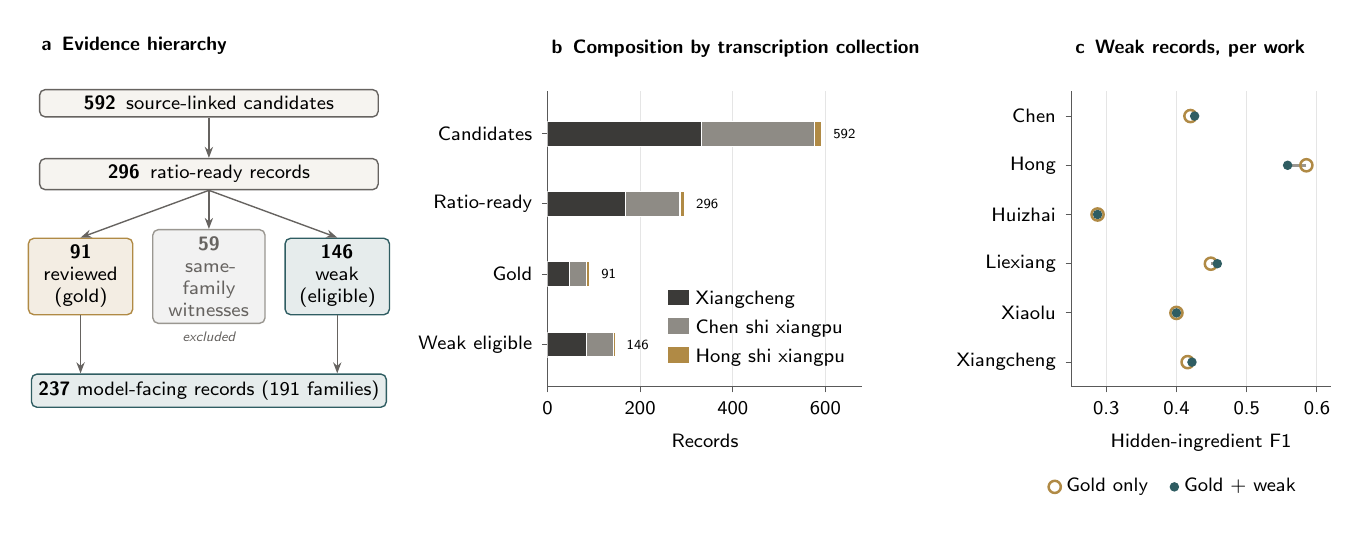
\begin{tikzpicture}
% ---------- panel a: evidence hierarchy ----------
\begin{scope}[box/.style={draw=cgray,rounded corners=2pt,fill=cpaper,font=\sffamily\sansmath\scriptsize,align=center,inner sep=2.5pt,line width=0.5pt},
              arr/.style={-{Stealth[length=4pt]},cgray,line width=0.5pt}]
\node[anchor=south west,font=\sffamily\sansmath\scriptsize] at (0,4.45) {\textbf{a}\enspace\textbf{Evidence hierarchy}};
\node[box,minimum width=4.3cm] (n1) at (2.25,3.95) {\textbf{592}\enspace source-linked candidates};
\node[box,minimum width=4.3cm] (n2) at (2.25,3.05) {\textbf{296}\enspace ratio-ready records};
\node[box,fill=cochre!15,draw=cochre,text width=1.15cm] (g) at (0.62,1.75) {\textbf{91}\\reviewed\\(gold)};
\node[box,fill=black!5,draw=clgray,text width=1.25cm,text=cgray] (x) at (2.25,1.75) {\textbf{59}\\same-family\\witnesses};
\node[box,fill=cteal!12,draw=cteal,text width=1.15cm] (w) at (3.88,1.75) {\textbf{146}\\weak\\(eligible)};
\node[font=\sffamily\sansmath\tiny\itshape,text=cgray] at (2.25,0.98) {excluded};
\node[box,fill=cteal!12,draw=cteal,minimum width=4.3cm] (m) at (2.25,0.3) {\textbf{237} model-facing records (191 families)};
\draw[arr] (n1) -- (n2);
\draw[arr] (n2.south) -- (g.north); \draw[arr] (n2.south) -- (x.north); \draw[arr] (n2.south) -- (w.north);
\draw[arr] (g.south) -- (m.north -| g.south); \draw[arr] (w.south) -- (m.north -| w.south);
\end{scope}
% ---------- panel b: composition by collection ----------
\begin{axis}[paper, at={(6.55cm,0.35cm)}, scale only axis, width=4.0cm, height=3.75cm,
  xbar stacked, bar width=9pt, xmin=0, xmax=680, ymin=0.4, ymax=4.6,
  ytick={1,2,3,4}, yticklabels={Weak eligible,Gold,Ratio-ready,Candidates},
  xtick={0,200,400,600}, xlabel={Records}, xmajorgrids,
  title={\textbf{b}\enspace\textbf{Composition by transcription collection}},
  legend style={at={(0.99,0.03)},anchor=south east,cells={anchor=west}}, legend cell align=left, reverse legend=false]
\addplot[fill=cdark,draw=white,line width=0.4pt] coordinates {(84,1) (47,2) (168,3) (332,4)};
\addplot[fill=cmid,draw=white,line width=0.4pt] coordinates {(58,1) (38,2) (118,3) (244,4)};
\addplot[fill=cochre,draw=white,line width=0.4pt] coordinates {(4,1) (6,2) (10,3) (16,4)};
\legend{Xiangcheng,Chen shi xiangpu,Hong shi xiangpu}
\node[font=\sffamily\sansmath\tiny,text=white] at (axis cs:166,4) {332};
\node[font=\sffamily\sansmath\tiny,text=white] at (axis cs:454,4) {244};
\node[font=\sffamily\sansmath\tiny,text=white] at (axis cs:84,3) {168};
\node[font=\sffamily\sansmath\tiny,text=white] at (axis cs:227,3) {118};
\node[font=\sffamily\sansmath\tiny,text=white] at (axis cs:42,1) {84};
\node[font=\sffamily\sansmath\tiny,text=white] at (axis cs:113,1) {58};
\node[font=\sffamily\sansmath\tiny,anchor=west] at (axis cs:596,4) {592};
\node[font=\sffamily\sansmath\tiny,anchor=west] at (axis cs:300,3) {296};
\node[font=\sffamily\sansmath\tiny,anchor=west] at (axis cs:95,2) {91};
\node[font=\sffamily\sansmath\tiny,anchor=west] at (axis cs:150,1) {146};
\end{axis}
% ---------- panel c: weak supervision per work ----------
\begin{axis}[paper, at={(13.2cm,0.35cm)}, scale only axis, width=3.3cm, height=3.75cm,
  xmin=0.25, xmax=0.62, ymin=0.5, ymax=6.5, ytick={1,...,6},
  yticklabels={Xiangcheng,Xiaolu,Liexiang,Huizhai,Hong,Chen},
  xtick={0.3,0.4,0.5,0.6}, xticklabel style={/pgf/number format/fixed}, xlabel={Hidden-ingredient F1}, xmajorgrids,
  title={\textbf{c}\enspace\textbf{Weak records, per work}},
  legend style={at={(0.4,-0.27)},anchor=north,legend columns=2,/tikz/every even column/.append style={column sep=6pt}}]
\draw[clgray,line width=1pt] (axis cs:0.4199,6)--(axis cs:0.4259,6) (axis cs:0.5850,5)--(axis cs:0.5583,5)
   (axis cs:0.4490,3)--(axis cs:0.4582,3) (axis cs:0.4159,1)--(axis cs:0.4221,1);
\addplot[only marks,mark=o,mark size=2.2pt,draw=cochre,line width=0.9pt] coordinates {(0.4199,6) (0.5850,5) (0.2877,4) (0.4490,3) (0.4000,2) (0.4159,1)};
\addplot[only marks,mark=*,mark size=1.5pt,color=cteal] coordinates {(0.4259,6) (0.5583,5) (0.2877,4) (0.4582,3) (0.4000,2) (0.4221,1)};
\legend{Gold only,Gold + weak}
\end{axis}
\end{tikzpicture}
\end{adjustwidth}
\caption{Evidence hierarchy and the weak-supervision test. (\textbf{a}) From 592 source-linked candidates to 237 model-facing records; witnesses of gold families are excluded before training. (\textbf{b}) Records per transcription collection at four stages; the gold bar counts formulas by the collection that transmits their work group. (\textbf{c}) Work-level hidden-ingredient F1 of SSCL trained on gold formulas only (open circles) or on gold plus weak records (filled circles), in the nested protocol of Section~\ref{sec:protocol}. Each point averages five masks within formula and then formulas within work. The work-averaged change is $-0.0009$ (exact sign-flip $p=1.0$).}
\label{fig:data}
\end{figure}

\begin{figure}[H]
\begin{adjustwidth}{-\extralength}{0cm}
\centering
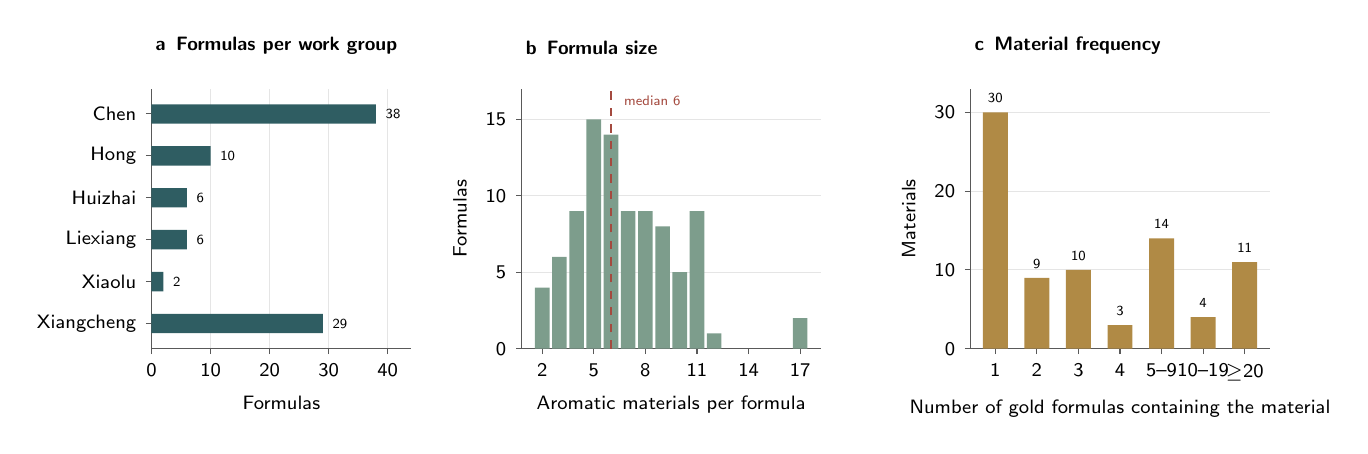
\begin{tikzpicture}
\begin{axis}[paper, at={(2.5cm,0)}, scale only axis, width=3.3cm, height=3.3cm,
  xbar, bar width=7pt, xmin=0, xmax=44, ymin=0.4, ymax=6.6, ytick={1,...,6},
  yticklabels={Xiangcheng,Xiaolu,Liexiang,Huizhai,Hong,Chen},
  xlabel={Formulas}, xmajorgrids, title={\textbf{a}\enspace\textbf{Formulas per work group}},
  nodes near coords, nodes near coords style={font=\sffamily\sansmath\tiny,anchor=west}, point meta=x]
\addplot[fill=cteal,draw=none] coordinates {(29,1) (2,2) (6,3) (6,4) (10,5) (38,6)};
\end{axis}
\begin{axis}[paper, at={(7.2cm,0)}, scale only axis, width=3.8cm, height=3.3cm,
  ybar, bar width=0.85, xmin=0.8, xmax=18.2, ymin=0, ymax=17, xtick={2,5,8,11,14,17},
  xlabel={Aromatic materials per formula}, ylabel={Formulas}, ymajorgrids,
  title={\textbf{b}\enspace\textbf{Formula size}}]
\addplot[fill=csage,draw=none] coordinates {(2,4) (3,6) (4,9) (5,15) (6,14) (7,9) (8,9) (9,8) (10,5) (11,9) (12,1) (17,2)};
\draw[cred,dashed,line width=0.7pt] (axis cs:6,0)--(axis cs:6,17);
\node[font=\sffamily\sansmath\tiny,text=cred,anchor=west] at (axis cs:6.2,16.2) {median 6};
\end{axis}
\begin{axis}[paper, at={(12.9cm,0)}, scale only axis, width=3.8cm, height=3.3cm,
  ybar, bar width=9pt, ymin=0, ymax=33, symbolic x coords={1,2,3,4,5--9,10--19,$\ge$20}, xtick=data,
  xlabel={Number of gold formulas containing the material}, ylabel={Materials}, ymajorgrids,
  title={\textbf{c}\enspace\textbf{Material frequency}},
  nodes near coords, nodes near coords style={font=\sffamily\sansmath\tiny}]
\addplot[fill=cochre,draw=none] coordinates {(1,30) (2,9) (3,10) (4,3) (5--9,14) (10--19,4) ($\ge$20,11)};
\end{axis}
\end{tikzpicture}
\end{adjustwidth}
\caption{The 91-formula gold reference set. (\textbf{a}) Formulas per work group. (\textbf{b}) Number of aromatic materials per formula; the dashed line marks the median of six. (\textbf{c}) Number of materials by how many gold formulas contain them; 30 of 81 materials occur once.}
\label{fig:corpus}
\end{figure}

%-----------------------------------------------------------------
\subsection{The Completion Task}
\label{sec:task}

\paragraph{Formulas as compositions.} For formula $i$ let $q_{ij}\ge0$ be the converted aromatic mass of material $j\in\{1,\dots,M\}$, $S_i=\{j:q_{ij}>0\}$ its support and $K_i=|S_i|$ its size. The closed composition~\cite{aitchison1982}
\begin{equation}
w_{ij}=\frac{q_{ij}}{\sum_{k\in S_i}q_{ik}},\qquad \bm w_i\in\Delta^{M-1},
\label{eq:closure}
\end{equation}
discards the arbitrary total batch size, which varies across books, and keeps relative proportions.

\paragraph{Observation and target.} The model sees an observed subset $O_i\subset S_i$ together with the reference fractions $\{w_{ij}:j\in O_i\}$; the hidden set is $H_i=S_i\setminus O_i$. It returns (i) a score $p_{ib}$ for each candidate $b\notin O_i$, (ii) a predicted size $\widehat K_i$ and hence a predicted hidden set $\widehat H_i$ of $\widehat K_i-|O_i|$ materials, and (iii) a completed composition $\widehat{\bm w}_i\in\Delta^{M-1}$ (Figure~\ref{fig:design}a). For a requested observed fraction $f$, the number of observed materials is
\begin{equation}
o(K,f)=\min\bigl\{K-1,\ \max[1,\operatorname{round}(fK)]\bigr\},
\label{eq:maskcount}
\end{equation}
computed on the materials of formula $i$ that belong to the training vocabulary of the fold, so at least one material is observed and at least one is hidden. Out-of-vocabulary materials always remain hidden.

\paragraph{Observation mechanisms.} Real damage is not uniform. Besides \emph{uniform} retention, we simulate \emph{abundance-biased} retention (probability of being observed proportional to reference mass, mimicking the survival of principal ingredients), \emph{source-prefix} retention (the first $o$ materials in source order, mimicking truncated copies), and uniform retention in which the count decoder is \emph{not told} $f$. In the terminology of missing-data theory~\cite{rubin1976}, the first and last mechanisms are completely at random with respect to material identity, whereas the abundance and prefix mechanisms are informative. The primary task uses uniform retention at $f=0.5$; secondary analyses use $f\in\{0.25,0.5,0.75\}$. Masks are generated from hashed seeds, and five masks per formula are used throughout.

\paragraph{Estimand.} Let $\overline{F}_{md}$ be the hidden-ingredient F1 of model $m$ (Section~\ref{sec:metrics}) averaged first over the five masks of each formula and then over the evaluated formulas of work $d$. The target of inference is the work-averaged difference from the frequency baseline,
\begin{equation}
\widehat\Delta_m=\frac1D\sum_{d=1}^{D}\Delta_{md},\qquad \Delta_{md}=\overline F_{md}-\overline F_{\mathrm{freq},d},\qquad D=6.
\label{eq:estimand}
\end{equation}
Equal weights answer the question ``how much does the method help for a new book?'' and prevent the two large groups (Chen and Xiangcheng, 67 of 90 evaluated formulas) from determining the result. The formula-weighted average is reported as a sensitivity analysis.

%-----------------------------------------------------------------
\subsection{Baselines: Frequency and the Directed Co-Formulation Graph}
\label{sec:baselines}

Let $X\in\{0,1\}^{N\times M}$ be the presence matrix of the $N$ training formulas and $c_b=\sum_iX_{ib}$. The \emph{frequency} baseline ranks candidates by the smoothed prevalence
\begin{equation}
\pi_b=\frac{c_b+\frac12}{N+1}.
\label{eq:prev}
\end{equation}
The \emph{directed graph} conditions on the observed materials. With $c_{ab}=\sum_iX_{ia}X_{ib}$, its edge is the smoothed conditional frequency
\begin{equation}
G_{ab}=\frac{c_{ab}+\alpha\pi_b}{c_a+\alpha},
\label{eq:graph}
\end{equation}
an estimate of $\Pr(b\in S\mid a\in S)$ shrunk toward $\pi_b$ with prior weight $\alpha$. It is asymmetric ($G_{ab}\neq G_{ba}$ in general): a common base material predicts little about a rare modifier, whereas the modifier may predict the base strongly. For any edge matrix $E$, the score of candidate $b$ is
\begin{equation}
p_{ib}=R\bigl(\{E_{ab}:a\in O_i\}\bigr),\qquad R\in\{\text{mean},\ \text{max},\ \text{mean of the top two}\},
\label{eq:reducer}
\end{equation}
where the reducer $R$ is a tuning parameter.

%-----------------------------------------------------------------
\subsection{Source-Stable Conditional Lift}
\label{sec:sscl}

The directed graph pools all training formulas as if they came from one book. If a pairing is common in one compilation because of a single editor's habit, the pooled edge will over-predict it in a new book. SSCL instead estimates every association inside each training work, puts the works on a common scale, and asks how consistently the association holds (Figure~\ref{fig:design}c).

\paragraph{Step 1: within-work conditionals.} For training work $d$ with $N_d$ formulas, let $c_{bd}$, $c_{ad}$ and $c_{abd}$ be the corresponding counts. Work prevalence is shrunk toward the global prevalence,
\begin{equation}
\pi_{bd}=\frac{c_{bd}+\kappa\pi_b}{N_d+\kappa},
\label{eq:workprev}
\end{equation}
and the within-work conditional probability $\theta_{abd}=\Pr(b\in S\mid a\in S,\ \text{work }d)$ receives a beta prior centred on $\pi_{bd}$. Its posterior mean is
\begin{equation}
\theta_{abd}\mid\text{data}\sim\operatorname{Beta}\bigl(c_{abd}+\alpha\pi_{bd},\ c_{ad}-c_{abd}+\alpha(1-\pi_{bd})\bigr),\qquad
\bar\theta_{abd}=\frac{c_{abd}+\alpha\pi_{bd}}{c_{ad}+\alpha}.
\label{eq:beta}
\end{equation}

\paragraph{Step 2: marginal-adjusted lift.} Books differ in how often they use each material. To compare associations across books we remove the work-specific base rate on the log-odds scale:
\begin{equation}
\ell_{abd}=\logit\bar\theta_{abd}-\logit\pi_{bd}.
\label{eq:lift}
\end{equation}
The lift is zero when $a$ carries no information about $b$ in work $d$. In particular, if $a$ never occurs in work $d$ ($c_{ad}=0$) then $\bar\theta_{abd}=\pi_{bd}$ and $\ell_{abd}=0$.

\paragraph{Step 3: pooling and dispersion.} Works in which $a$ is rarely observed carry little information about its associations. With exposure weights $v_{ad}=c_{ad}/(c_{ad}+\alpha)\in[0,1)$, which vanish for works where $a$ is absent,
\begin{equation}
\mu_{ab}=\frac{\sum_dv_{ad}\ell_{abd}}{\sum_dv_{ad}},\qquad
s_{ab}^2=\frac{\sum_dv_{ad}\bigl(\ell_{abd}-\mu_{ab}\bigr)^2}{\sum_dv_{ad}}.
\label{eq:pool}
\end{equation}

\paragraph{Step 4: transport and penalise.} The prevalence of $b$ in the target book is unknown, so the pooled lift is added to the global log-odds, and the spread is subtracted:
\begin{equation}
G^{\star}_{ab}=\expit\bigl(\logit\pi_b+\mu_{ab}-\gamma s_{ab}\bigr),\qquad
G^{\mathrm{SS}}_{ab}=(1-\lambda)\,G_{ab}+\lambda\,G^{\star}_{ab},
\label{eq:sscl}
\end{equation}
with $\expit(x)=1/(1+e^{-x})$. The blend weight $\lambda$ keeps the direct graph as a fallback for materials with little within-work support. Candidates are scored by Equation~\eqref{eq:reducer} with $E=G^{\mathrm{SS}}$. The shrinkage constant is fixed at $\kappa=5$; $\alpha$, $\gamma$, $\lambda$ and the reducer are selected by inner validation.

The following statement makes the role of the penalty precise.

\begin{xprop}[Robust-edge representation]
\label{prop:robust}
Let $\mathcal U_{ab}(\gamma)=\{\ell:|\ell-\mu_{ab}|\le\gamma s_{ab}\}$. Then
\begin{equation}
G^{\star}_{ab}=\min_{\ell\in\mathcal U_{ab}(\gamma)}\expit\bigl(\logit\pi_b+\ell\bigr).
\label{eq:robust}
\end{equation}
If, in addition, the lift of the unseen target work satisfies $\ell_{ab,d^\star}\sim\mathcal N(\mu_{ab},s_{ab}^2)$, then
\begin{equation*}
\Pr\bigl\{\expit(\logit\pi_b+\ell_{ab,d^\star})\ge G^\star_{ab}\bigr\}=\Phi(\gamma),
\end{equation*}
where $\Phi$ is the standard normal distribution function.
\end{xprop}
\begin{xproof}
$\expit$ is strictly increasing, so the minimum over the interval is attained at its lower endpoint $\mu_{ab}-\gamma s_{ab}$. Under the normal model, $\Pr(\ell_{ab,d^\star}\ge\mu_{ab}-\gamma s_{ab})=\Phi(\gamma)$, and monotonicity transfers the event to the edge scale.
\end{xproof}

Thus $G^\star$ is a distributionally robust~\cite{bental2009} edge: it assumes the least favourable plausible lift for the new book. Under the random-effects reading it is a lower predictive quantile; the grid $\gamma\in\{0,0.25,0.5,1\}$ corresponds to quantile levels $0.50$, $0.60$, $0.69$ and $0.84$. Setting $\gamma=0$ gives a pooled lift without penalty, $\lambda=0$ recovers the direct graph, and a material observed in only one training work has $s_{ab}=0$.

\begin{xrem}
\label{rem:dispersion}
In a random-effects model $\ell_{abd}=\ell_{ab}+u_{abd}+e_{abd}$ with between-work effect $u_{abd}$ (variance $\tau_{ab}^2$) and estimation error $e_{abd}$ (variance $\varsigma_{abd}^2$), the dispersion $s_{ab}^2$ in Equation~\eqref{eq:pool} estimates approximately $\tau_{ab}^2$ plus a weighted average of the $\varsigma_{abd}^2$. The penalty therefore combines genuine heterogeneity with sampling noise, which makes it conservative for poorly supported edges. A moment estimator of the DerSimonian--Laird type~\cite{dersimonian1986} would separate the two components. Moreover, with at most five training works the relative standard error of a standard deviation is roughly $1/\sqrt{2(D-1)}\approx0.35$ under normality, so the penalty re-ranks candidates using a noisy quantity. Section~\ref{sec:disc-penalty} returns to this point.
\end{xrem}

%-----------------------------------------------------------------
\subsection{Provenance-Aware Weak Supervision}
\label{sec:weak}

Let $z_i\in\{\text{gold},\text{weak}\}$ be the evidence class of record $i$, $\fmly(i)$ its genealogy family, $C(i)$ its transcription collection, and $|\fmly|$ the number of weak records in family $\fmly$ across all collections. Records receive the weights
\begin{equation}
\omega_i(\eta)=\begin{cases}1,& z_i=\text{gold},\\ \eta/|\fmly(i)|,& z_i=\text{weak},\end{cases}\qquad \eta\in\{0,0.1,0.25,0.5,1\},
\label{eq:weights}
\end{equation}
and every count in Sections~\ref{sec:baselines}--\ref{sec:sscl} is replaced by its weighted version, for example $c_b^{(\omega)}=\sum_i\omega_iX_{ib}$, $c_{ab}^{(\omega)}=\sum_i\omega_iX_{ia}X_{ib}$ and $N^{(\omega)}=\sum_i\omega_i$. The size histogram, the EASE Gram matrix and the composition neighbours use the same weights. Each weak collection enters SSCL as an additional source domain.

For an outer test work $d^\star$ with families $\mathcal F_{d^\star}$, the admissible weak pool is
\begin{equation}
\mathcal W_{d^\star}=\bigl\{i:\ z_i=\text{weak},\ C(i)\neq C(d^\star),\ \fmly(i)\notin\mathcal F_{d^\star}\bigr\}.
\label{eq:pool-weak}
\end{equation}
The same rule is applied to every inner validation work. The weight $\eta$ is selected jointly with the model hyper-parameters by inner validation.

\begin{xprop}[Family budget]
\label{prop:budget}
For every family $\fmly$, the total weight of its admissible members is $\sum_{i\in\fmly\cap\mathcal W_{d^\star}}\omega_i=\eta\,|\fmly\cap\mathcal W_{d^\star}|/|\fmly|\le\eta$. Consequently the effective weak mass
\begin{equation}
N^{\mathrm{eff}}_{\mathrm{weak}}(d^\star)=\sum_{i\in\mathcal W_{d^\star}}\omega_i
\label{eq:effmass}
\end{equation}
is at most $\eta$ times the number of families represented in $\mathcal W_{d^\star}$, and $\eta=0$ reproduces gold-only training exactly.
\end{xprop}
\begin{xproof}
Sum Equation~\eqref{eq:weights} over the admissible members of $\fmly$; the ratio of admissible to total members is at most one. For $\eta=0$ all weak weights vanish and every weighted count equals its gold-only value.
\end{xproof}

With $\eta\le1$, a family of copied witnesses can therefore never weigh more than one reviewed formula, and a family whose members are partly blocked by the collection rule contributes proportionally less.

%-----------------------------------------------------------------
\subsection{Item-Based Comparators}
\label{sec:items}

Three standard recommender models test whether other ways of exploiting item dependencies do better. EASE~\cite{steck2019} learns a dense item-to-item matrix in closed form: with $W=\operatorname{diag}(\omega)$ and $\Omega=(X^\top WX+\rho I)^{-1}$, $B_{ab}=-\Omega_{ab}/\Omega_{bb}$ for $a\ne b$ and $B_{bb}=0$. A SLIM-type model~\cite{ning2011} estimates a sparse non-negative matrix with zero diagonal,
\begin{equation}
\widehat B=\arg\min_{B\ge0,\ \operatorname{diag}B=0}\ \frac1{2N}\lVert X-XB\rVert_F^2+\nu\Bigl[\xi\lVert B\rVert_1+\frac{1-\xi}{2}\lVert B\rVert_F^2\Bigr].
\label{eq:slim}
\end{equation}
For both, the score is the observed indicator vector multiplied by $B$, with a small prevalence tie-breaker. Personalised PageRank (PPR)~\cite{page1999} diffuses from the observed materials over the row-normalised direct graph $Q$: $\bm z^{(t+1)}=(1-\delta)\bm u_i+\delta\,\bm z^{(t)}Q$ with restart vector $\bm u_i$ supported on $O_i$, iterated 50 times. Formula $k$-nearest neighbours~\cite{cover1967} and PureSVD~\cite{cremonesi2010} are included in the secondary protocol.

%-----------------------------------------------------------------
\subsection{Formula Size and Composition}
\label{sec:count}

All ranking models share one size model and one composition rule, so that differences in F1 reflect ranking alone.

\paragraph{Size.} Let $n_k$ be the (weighted) number of training formulas with $k$ materials and $K_{\max}$ the largest training size. The size prior and its posterior given $|O_i|=o$ and known $f$ are
\begin{equation}
p_0(k)=\frac{n_k+\frac12}{N+K_{\max}/2},\quad k=1,\dots,K_{\max};\qquad
p(k\mid o,f)\propto p_0(k)\,\mathbf 1\{o(k,f)=o\}.
\label{eq:count}
\end{equation}
The indicator encodes the masking rule~\eqref{eq:maskcount}, which already implies $k\ge o+1$. The prediction $\widehat K_i$ is the posterior median, and the top $\widehat K_i-o$ candidates form $\widehat H_i$. When $f$ is withheld, the decoder must infer $K_i$ from $o$ and the size prior alone, which is harder. Central 80\% posterior intervals $[L_i,U_i]$ are recalibrated with split conformal prediction~\cite{lei2018,angelopoulos2023} using the non-conformity score $e_i=\max\{L_i-K_i,\ K_i-U_i,\ 0\}$ on development-work-held-out instances; with $n$ calibration instances the interval is widened by the empirical quantile of $e$ at level $\lceil(n+1)(0.8)\rceil/n$.

\paragraph{Composition.} Observed fractions are kept, and the residual mass $m_i=1-\sum_{a\in O_i}w_{ia}$ is divided among the predicted hidden materials in proportion to a non-negative ratio score $R_{ib}$ derived from the ten training formulas most similar to the observed part:
\begin{equation}
\widehat w_{ib}=\begin{cases}w_{ib},& b\in O_i,\\ m_iR_{ib}\big/\sum_{h\in\widehat H_i}R_{ih},& b\in\widehat H_i,\\ 0,&\text{otherwise.}\end{cases}
\label{eq:composition}
\end{equation}

%-----------------------------------------------------------------
\subsection{Probability Calibration}
\label{sec:calib}

Graph scores are not probabilities. For each outer fold we fit, on inner held-out-work predictions only, a temperature map and a two-parameter logistic (Platt-type) map~\cite{guo2017,platt1999},
\begin{equation}
p^{(t)}=\expit\bigl(\logit(p)/t\bigr),\qquad p^{(L)}=\expit\bigl(a\logit(p)+c\bigr),\quad a>0,
\label{eq:calib}
\end{equation}
by minimising candidate-level negative log-likelihood. The temperature map rescales log-odds about zero; the logistic map can also shift them. The outer test work contributes no calibration labels.

%-----------------------------------------------------------------
\subsection{Evaluation Protocol}
\label{sec:protocol}

\paragraph{Primary protocol: nested leave-one-work-out.} Each of the six work groups serves once as the outer test work (Figure~\ref{fig:design}b). The test work is absent from vocabulary construction, prevalence and edge estimation, hyper-parameter selection and calibration. Inside the remaining five works, leave-one-work-out validation selects the configuration with the highest work-averaged hidden F1 (weighted Jaccard breaks ties), which is then refitted on all five works and applied to the test work. Nesting prevents selection bias in the reported error~\cite{varma2006}; blocking by work follows the recommendation for grouped data~\cite{roberts2017} and the logic of domain-shift benchmarks~\cite{koh2021,wu2023}. The grids are: direct graph $\alpha\in\{0.5,1,2,5\}$; SSCL $\alpha\in\{1,2,5\}$, $\gamma\in\{0,0.25,0.5,1\}$, $\lambda\in\{0.25,0.5,0.75,1\}$ and mean or maximum reduction; EASE $\rho$ from 1 to 1000; SLIM four values of $\nu$ and three of $\xi$; PPR five values of $\delta$.

\paragraph{Weak-supervision experiment.} The full nested protocol is repeated for the directed graph and SSCL with $\eta$ added to the inner search. The admissible pool~\eqref{eq:pool-weak} is rebuilt for every inner and outer target, giving 62 to 142 admissible weak records per outer fold.

\paragraph{Secondary protocol: two works held out.} During development, five of the six work groups (85 formulas) were used; configurations were selected by leave-one-work-out validation and evaluated on all ten pairs of held-out works. This harder protocol removes two books at once and is used for the comparator panel, the near-duplicate test, the rarity analysis and the size intervals.

\begin{figure}[H]
\begin{adjustwidth}{-\extralength}{0cm}
\centering
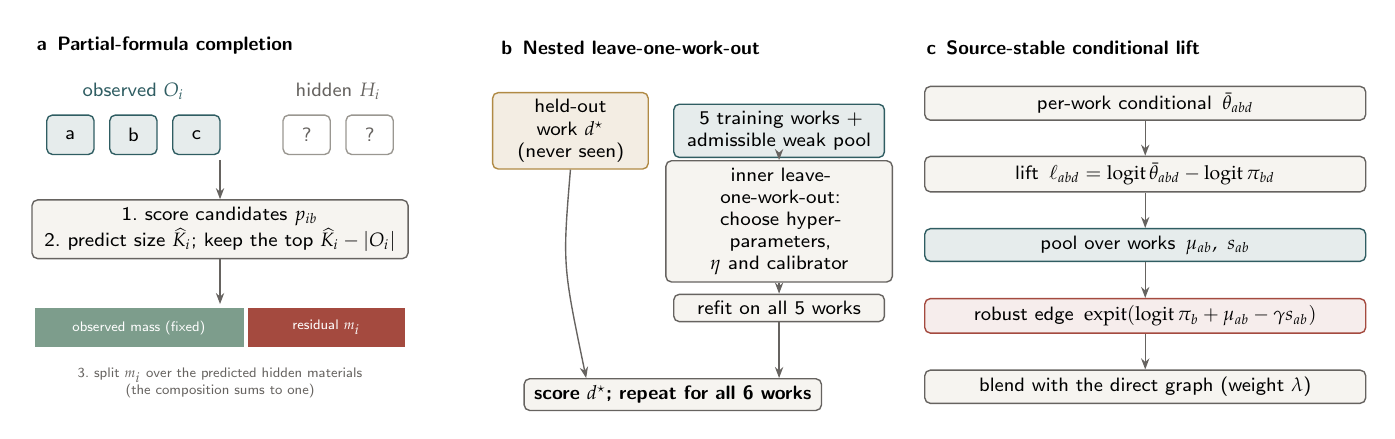
\begin{tikzpicture}[box/.style={draw=cgray,rounded corners=2pt,fill=cpaper,font=\sffamily\scriptsize,align=center,inner sep=2.5pt,line width=0.5pt},
  arr/.style={-{Stealth[length=4pt]},cgray,line width=0.5pt}]
% panel a
\node[anchor=south west,font=\sffamily\scriptsize] at (0,4.55) {\textbf{a}\enspace\textbf{Partial-formula completion}};
\node[font=\sffamily\scriptsize,text=cteal] at (1.35,4.2) {observed $O_i$};
\node[font=\sffamily\scriptsize,text=cgray] at (3.95,4.2) {hidden $H_i$};
\foreach \x/\t in {0.55/a,1.35/b,2.15/c}{\node[box,fill=cteal!12,draw=cteal,minimum width=0.6cm,minimum height=0.5cm] at (\x,3.65) {\t};}
\foreach \x in {3.55,4.35}{\node[box,fill=white,draw=clgray,minimum width=0.6cm,minimum height=0.5cm,text=cgray] at (\x,3.65) {?};}
\node[box,text width=4.6cm] (s) at (2.45,2.45) {1.\ score candidates $p_{ib}$\\2.\ predict size $\widehat K_i$; keep the top $\widehat K_i-|O_i|$};
\draw[arr] (2.45,3.33) -- (s.north);
\fill[csage] (0.1,0.95) rectangle (2.75,1.45); \fill[cred] (2.8,0.95) rectangle (4.8,1.45);
\node[font=\sffamily\tiny,text=white] at (1.42,1.2) {observed mass (fixed)};
\node[font=\sffamily\tiny,text=white] at (3.8,1.2) {residual $m_i$};
\draw[arr] (s.south) -- (2.45,1.5);
\node[font=\sffamily\tiny,text=cgray,align=center] at (2.45,0.5) {3.\ split $m_i$ over the predicted hidden materials\\(the composition sums to one)};
% panel b
\begin{scope}[xshift=5.9cm]
\node[anchor=south west,font=\sffamily\scriptsize] at (0,4.55) {\textbf{b}\enspace\textbf{Nested leave-one-work-out}};
\node[box,fill=cochre!15,draw=cochre,text width=1.8cm] (t) at (1.0,3.7) {held-out work $d^\star$\\(never seen)};
\node[box,fill=cteal!12,draw=cteal,text width=2.5cm] (tr) at (3.65,3.7) {5 training works +\\admissible weak pool};
\node[box,text width=2.7cm] (in) at (3.65,2.55) {inner leave-one-work-out:\\choose hyper-parameters,\\$\eta$ and calibrator};
\node[box,text width=2.5cm] (rf) at (3.65,1.45) {refit on all 5 works};
\node[box,text width=3.6cm,font=\sffamily\scriptsize\bfseries] (sc) at (2.3,0.35) {score $d^\star$; repeat for all 6 works};
\draw[arr] (tr) -- (in); \draw[arr] (in) -- (rf); \draw[arr] (rf.south) -- (sc.north -| rf.south);
\draw[arr] (t.south) .. controls (0.9,2.0) .. (sc.north -| 1.2,0);
\end{scope}
% panel c
\begin{scope}[xshift=11.3cm]
\node[anchor=south west,font=\sffamily\scriptsize] at (0,4.55) {\textbf{c}\enspace\textbf{Source-stable conditional lift}};
\node[box,minimum width=5.6cm] (c1) at (2.9,4.05) {per-work conditional\enspace $\bar\theta_{abd}$};
\node[box,minimum width=5.6cm] (c2) at (2.9,3.15) {lift\enspace $\ell_{abd}=\operatorname{logit}\bar\theta_{abd}-\operatorname{logit}\pi_{bd}$};
\node[box,minimum width=5.6cm,fill=cteal!12,draw=cteal] (c3) at (2.9,2.25) {pool over works\enspace $\mu_{ab},\ s_{ab}$};
\node[box,minimum width=5.6cm,fill=cred!10,draw=cred] (c4) at (2.9,1.35) {robust edge\enspace $\operatorname{expit}(\operatorname{logit}\pi_b+\mu_{ab}-\gamma s_{ab})$};
\node[box,minimum width=5.6cm] (c5) at (2.9,0.45) {blend with the direct graph (weight $\lambda$)};
\draw[arr] (c1)--(c2); \draw[arr] (c2)--(c3); \draw[arr] (c3)--(c4); \draw[arr] (c4)--(c5);
\end{scope}
\end{tikzpicture}
\end{adjustwidth}
\caption{Task, protocol and method. (\textbf{a}) The model sees some materials with their reference mass fractions, scores all other materials, predicts the formula size, and divides the residual mass among the selected materials. (\textbf{b}) Nested leave-one-work-out evaluation: hyper-parameters, the weak-label weight $\eta$ and the probability calibrator are chosen by inner validation on the five training works; the held-out work is scored once. (\textbf{c}) Source-stable conditional lift (Equations~\eqref{eq:workprev}--\eqref{eq:sscl}).}
\label{fig:design}
\end{figure}

%-----------------------------------------------------------------
\subsection{Metrics}
\label{sec:metrics}

\paragraph{Set recovery.} With $\widehat H_i$ the predicted and $H_i$ the true hidden set,
\begin{equation}
P_i=\frac{|H_i\cap\widehat H_i|}{|\widehat H_i|},\qquad R_i=\frac{|H_i\cap\widehat H_i|}{|H_i|},\qquad F_{1,i}=\frac{2P_iR_i}{P_i+R_i},
\label{eq:f1}
\end{equation}
with $F_{1,i}=0$ when $P_i=R_i=0$. Size error is $|\widehat K_i-K_i|$.

\paragraph{Composition.} The weighted Jaccard similarity~\cite{ioffe2010} of two compositions is
\begin{equation}
J^{w}_i=\frac{\sum_j\min(w_{ij},\widehat w_{ij})}{\sum_j\max(w_{ij},\widehat w_{ij})}.
\label{eq:wj}
\end{equation}

\begin{xlem}
\label{lem:wj}
For $\bm w,\widehat{\bm w}\in\Delta^{M-1}$ with total-variation distance $\TV=\frac12\sum_j|w_j-\widehat w_j|$,
\begin{equation}
J^{w}=\frac{1-\TV}{1+\TV}.
\label{eq:wjtv}
\end{equation}
If $\widehat{\bm w}$ is produced by rule~\eqref{eq:composition}, then $\TV\le m_i$ and hence $J^w_i\ge(1-m_i)/(1+m_i)$, whatever materials are selected.
\end{xlem}
\begin{xproof}
Since $\min(x,y)+\max(x,y)=x+y$ and $\max(x,y)-\min(x,y)=|x-y|$, summing over $j$ gives $\sum\min+\sum\max=2$ and $\sum\max-\sum\min=2\TV$, so $\sum\min=1-\TV$ and $\sum\max=1+\TV$. Under rule~\eqref{eq:composition} the observed coordinates agree and both vectors place mass $m_i$ on the remaining coordinates, so $\sum_{j\notin O_i}|w_{ij}-\widehat w_{ij}|\le2m_i$.
\end{xproof}

Lemma~\ref{lem:wj} shows that weighted Jaccard is a monotone transform of total variation, and that part of it is guaranteed by the observed input: with half of a typical formula's mass observed ($m_i=0.5$) the score cannot fall below $1/3$. Weighted Jaccard should therefore be compared across models on the same masks, never against zero, and the quantity $1-\TV_i/m_i\in[0,1]$ isolates what the model earns on the hidden mass.

\paragraph{Calibration.} For candidate labels $y_n\in\{0,1\}$ and probabilities $p_n$, $n=1,\dots,L$, we report the Brier score~\cite{brier1950}, the negative log-likelihood and the adaptive calibration error~\cite{nixon2019},
\begin{align}
\mathrm{Brier}&=\frac1L\sum_n(p_n-y_n)^2,\qquad
\mathrm{NLL}=-\frac1L\sum_n\bigl[y_n\log p_n+(1-y_n)\log(1-p_n)\bigr],\nonumber\\
\mathrm{ACE}&=\sum_{g}\frac{|I_g|}{L}\Bigl|\frac1{|I_g|}\sum_{n\in I_g}(p_n-y_n)\Bigr|,
\label{eq:calmetrics}
\end{align}
where the $I_g$ are equal-count probability groups within each work. Brier score and NLL are averaged within formula, then within work; all three are then averaged over works.

%-----------------------------------------------------------------
\subsection{Statistical Inference with Six Works}
\label{sec:inference}

Formulas from the same work are dependent, and masks of the same formula are repeated measurements, so neither is an independent replicate. We therefore treat the six work-level differences $\Delta_{md}$ as the data. Under the null hypothesis that each $\Delta_{md}$ is symmetrically distributed about zero, the exact two-sided sign-flip (randomisation) test~\cite{fisher1935} has
\begin{equation}
p_{\mathrm{flip}}=2^{-D}\sum_{\bm s\in\{-1,1\}^D}\mathbf 1\Bigl\{\Bigl|\frac1D\sum_ds_d\Delta_{md}\Bigr|\ge|\widehat\Delta_m|\Bigr\}.
\label{eq:signflip}
\end{equation}
Few clusters limit what any test can show~\cite{cameron2008}, and the next statement quantifies the limit.

\begin{xprop}[Attainable $p$-value floor]
\label{prop:floor}
If $D'$ of the $D$ differences are non-zero, then $p_{\mathrm{flip}}\ge2^{1-D'}$. With $D=6$ and one tie, $p_{\mathrm{flip}}\ge0.0625$ however large the effect.
\end{xprop}
\begin{xproof}
The identity assignment and the global sign flip both give statistics equal to $|\widehat\Delta_m|$. Flipping the sign of a zero difference does not change the statistic, so each of these two patterns is repeated $2^{D-D'}$ times. Hence at least $2\cdot2^{D-D'}$ of the $2^D$ assignments meet the condition in Equation~\eqref{eq:signflip}.
\end{xproof}

A test at the 5\% level was therefore impossible for the pre-specified primary comparison once one work tied, and we do not replace it by a one-sided or formula-level test after the fact. Instead we report, in addition to $p_{\mathrm{flip}}$, the 90\% confidence interval obtained by inverting the test,
\begin{equation}
\mathcal C_{0.90}=\bigl\{\theta:\ p_{\mathrm{flip}}(\Delta_{m1}-\theta,\dots,\Delta_{mD}-\theta)>0.10\bigr\},
\label{eq:ci}
\end{equation}
which is valid under symmetry of the differences about $\theta$, together with the formula-weighted estimate and the range of leave-one-work-out means.

The comparison of SSCL with frequency on hidden F1 in the primary protocol was designated as primary. The directed graph against frequency, SSCL against the directed graph, and weak-augmented against gold-only SSCL are secondary comparisons. All other analyses are descriptive.

%-----------------------------------------------------------------
\subsection{Diagnostics}
\label{sec:diagnostics}

\paragraph{Near duplicates.} A formula is a cross-work near duplicate if $\max_{r:\,d_r\ne d_i}|S_i\cap S_r|/|S_i\cup S_r|\ge0.8$. The secondary protocol is repeated after removing such formulas.

\paragraph{Rarity and stability.} Hidden-material recall is stratified by the number of training formulas containing the material (absent, one, two to four, at least five). Stability is the mean pairwise Jaccard similarity of the five predicted hidden sets of a formula.

\paragraph{Case study.} One formula is displayed in full. From the six Hong formulas under mask seed 17, we select the formula whose hidden F1 is closest to the median, breaking ties by identifier.

The chemical-similarity analysis and the computational profile are described in Appendix~\ref{app:dev}; notation is summarised in Table~\ref{tab:notation}.

%=================================================================
\section{Results}
\label{sec:results}

\subsection{Conditional Co-Formulation Transfers Across Books}
\label{sec:main}

Table~\ref{tab:main} summarises the primary protocol. All structured models exceed frequency on precision, recall, hidden F1 and weighted Jaccard. SSCL reached a work-averaged hidden F1 of 0.426 against 0.378 for frequency, and the directed graph reached the same value. EASE attained the highest weighted Jaccard (0.473), closely followed by SSCL (0.472). SLIM gained least over frequency. Size error is identical across models by construction.

\begin{table}[H]
\caption{Primary protocol: nested leave-one-work-out completion at 50\% uniform observation. Entries are unweighted means of six work-level means (90 evaluated formulas, five masks each). All models share the size module, hence the common size error.}
\label{tab:main}
\small
\begin{tabularx}{\textwidth}{lCCCCC}
\toprule
\textbf{Model} & \textbf{Precision} & \textbf{Recall} & \textbf{Hidden F1} & \textbf{Weighted Jaccard} & \textbf{Size MAE} \\
\midrule
Frequency & 0.432 & 0.363 & 0.378 & 0.451 & 1.145 \\
Directed graph & 0.481 & 0.413 & 0.426 & 0.470 & 1.145 \\
SSCL & 0.480 & 0.414 & \textbf{0.426} & 0.472 & 1.145 \\
EASE & 0.479 & 0.408 & 0.423 & \textbf{0.473} & 1.145 \\
SLIM & 0.440 & 0.371 & 0.387 & 0.455 & 1.145 \\
PPR & 0.467 & 0.397 & 0.412 & 0.459 & 1.145 \\
\bottomrule
\end{tabularx}
\end{table}

The gain is consistent across books (Table~\ref{tab:works-f1}, Figure~\ref{fig:performance}). SSCL and the directed graph improved on frequency in five works and tied in Xiaolu, which contributes only two formulas. The largest gains occurred in the Hong group (SSCL $+0.116$), and Huizhai remained the hardest group for every model (F1 below 0.29).

\begin{table}[H]
\caption{Hidden F1 by held-out work in the primary protocol. $n$ is the number of evaluated formulas; each formula score averages five masks.}
\label{tab:works-f1}
\small
\begin{tabularx}{\textwidth}{lcCCCC}
\toprule
\textbf{Held-out work} & $\bm n$ & \textbf{Frequency} & \textbf{Directed graph} & \textbf{SSCL} & \textbf{EASE} \\
\midrule
Chen & 38 & 0.3812 & 0.4268 & 0.4199 & 0.4135 \\
Hong & 6 & 0.4689 & 0.5583 & 0.5850 & 0.5717 \\
Huizhai & 9 & 0.2268 & 0.2877 & 0.2877 & 0.2867 \\
Liexiang & 6 & 0.4365 & 0.4649 & 0.4490 & 0.4588 \\
Xiaolu & 2 & 0.4000 & 0.4000 & 0.4000 & 0.3833 \\
Xiangcheng & 29 & 0.3557 & 0.4180 & 0.4159 & 0.4232 \\
\bottomrule
\end{tabularx}
\end{table}

Table~\ref{tab:inference} gives the work-level inference. For the primary comparison the mean difference is 0.048 with exact $p_{\mathrm{flip}}=0.0625$, which by Proposition~\ref{prop:floor} is the smallest value the design could produce after the Xiaolu tie. The 90\% sign-flip interval, 0.013 to 0.088, excludes zero. The formula-weighted estimate (0.050) and the leave-one-work-out means (0.035 to 0.058) show that the result depends neither on the weighting nor on any single book. SSCL and the directed graph differ by 0.0003 ($p=1.0$), and the 90\% interval ($-0.009$ to $0.013$) bounds the effect of the dispersion penalty to about one hundredth of F1 in either direction. Five of the six outer folds selected a positive penalty $\gamma$, so the null result reflects an inert penalty rather than a penalty that was never chosen.

\begin{table}[H]
\caption{Work-level inference for hidden F1 (primary protocol, $D=6$ works). The column $+/0/-$ counts works that improve, tie and worsen. $p$ is the exact two-sided sign-flip $p$-value (Equation~\eqref{eq:signflip}); the interval inverts the same test (Equation~\eqref{eq:ci}). LOWO: range of the mean after leaving out one work.}
\label{tab:inference}
\small
\begin{adjustwidth}{-\extralength}{0cm}
\begin{tabularx}{\linewidth}{Lcccccc}
\toprule
\textbf{Comparison} & \textbf{Mean $\bm{\widehat\Delta}$} & \textbf{Formula-weighted} & $\bm{+/0/-}$ & $\bm p$ & \textbf{90\% interval} & \textbf{LOWO range} \\
\midrule
SSCL $-$ frequency (primary) & 0.048 & 0.050 & 5/1/0 & 0.0625 & [0.013, 0.088] & [0.035, 0.058] \\
Directed graph $-$ frequency & 0.048 & 0.053 & 5/1/0 & 0.0625 & [0.023, 0.075] & [0.039, 0.057] \\
EASE $-$ frequency & 0.045 & 0.049 & 5/0/1 & 0.0625 & [0.008, 0.081] & [0.033, 0.057] \\
SSCL $-$ directed graph & 0.000 & $-$0.003 & 1/2/3 & 1.000 & [$-$0.009, 0.013] & --- \\
SSCL weak $-$ SSCL gold & $-$0.001 & --- & 3/2/1 & 1.000 & [$-$0.013, 0.008] & --- \\
\bottomrule
\end{tabularx}
\end{adjustwidth}
\end{table}

\begin{figure}[H]
\begin{adjustwidth}{-\extralength}{0cm}
\centering
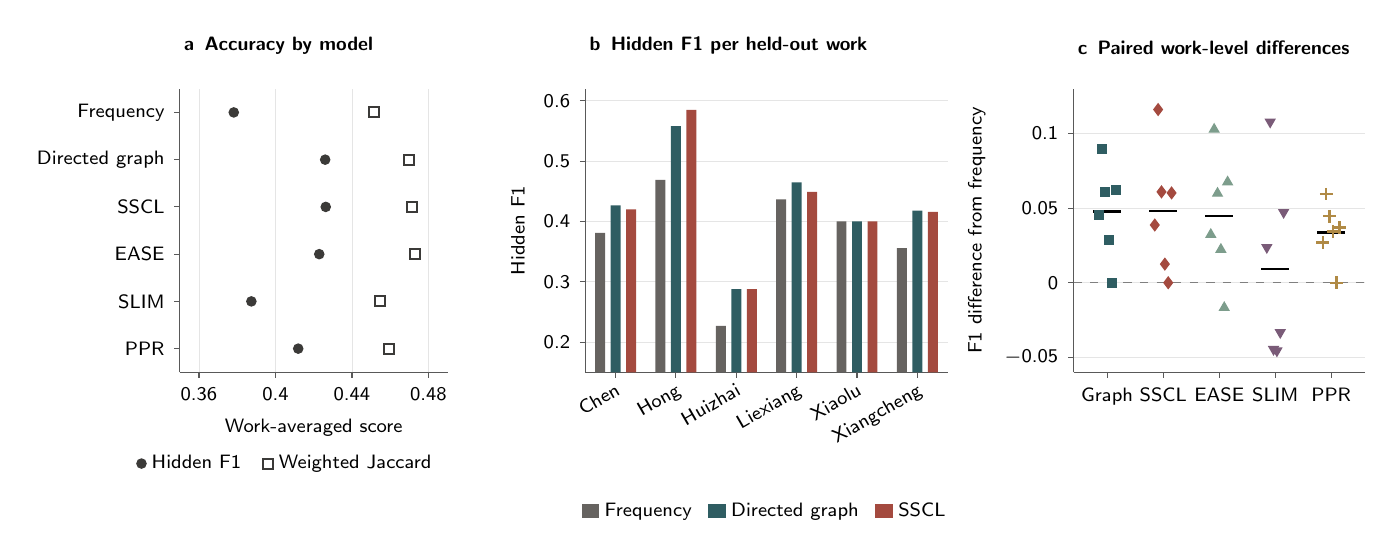
\begin{tikzpicture}
\begin{axis}[paper, at={(1.75cm,0)}, scale only axis, width=3.4cm, height=3.6cm,
  xmin=0.35, xmax=0.49, ymin=0.5, ymax=6.5, ytick={1,...,6},
  yticklabels={PPR,SLIM,EASE,SSCL,Directed graph,Frequency},
  xtick={0.36,0.40,0.44,0.48}, xticklabel style={/pgf/number format/fixed,/pgf/number format/precision=2},
  xlabel={Work-averaged score}, xmajorgrids, title={\textbf{a}\enspace\textbf{Accuracy by model}},
  legend style={at={(0.4,-0.25)},anchor=north,legend columns=2,/tikz/every even column/.append style={column sep=6pt}}]
\addplot[only marks,mark=*,mark size=1.7pt,color=cdark] coordinates {(0.3782,6) (0.4260,5) (0.4263,4) (0.4229,3) (0.3874,2) (0.4119,1)};
\addplot[only marks,mark=square,mark size=1.8pt,draw=cdark,line width=0.7pt] coordinates {(0.4514,6) (0.4699,5) (0.4716,4) (0.4730,3) (0.4545,2) (0.4594,1)};
\legend{Hidden F1,Weighted Jaccard}
\end{axis}
\begin{axis}[paper, at={(6.9cm,0)}, scale only axis, width=4.6cm, height=3.6cm,
  ybar, bar width=3.6pt, ymin=0.15, ymax=0.62, ytick={0.2,0.3,0.4,0.5,0.6},
  yticklabel style={/pgf/number format/fixed,/pgf/number format/precision=1},
  symbolic x coords={Chen,Hong,Huizhai,Liexiang,Xiaolu,Xiangcheng}, xtick=data,
  x tick label style={rotate=30,anchor=north east,inner sep=1pt}, enlarge x limits=0.1,
  ylabel={Hidden F1}, ymajorgrids, title={\textbf{b}\enspace\textbf{Hidden F1 per held-out work}},
  legend style={at={(0.5,-0.42)},anchor=north,legend columns=3,/tikz/every even column/.append style={column sep=4pt}}, legend image code/.code={\draw[#1,draw=none] (0cm,-0.08cm) rectangle (0.22cm,0.1cm);}]
\addplot[fill=cgray,draw=none] coordinates {(Chen,0.3812) (Hong,0.4689) (Huizhai,0.2268) (Liexiang,0.4365) (Xiaolu,0.4000) (Xiangcheng,0.3557)};
\addplot[fill=cteal,draw=none] coordinates {(Chen,0.4268) (Hong,0.5583) (Huizhai,0.2877) (Liexiang,0.4649) (Xiaolu,0.4000) (Xiangcheng,0.4180)};
\addplot[fill=cred,draw=none] coordinates {(Chen,0.4199) (Hong,0.5850) (Huizhai,0.2877) (Liexiang,0.4490) (Xiaolu,0.4000) (Xiangcheng,0.4159)};
\legend{Frequency,Directed graph,SSCL}
\end{axis}
\begin{axis}[paper, at={(13.1cm,0)}, scale only axis, width=3.7cm, height=3.6cm,
  xmin=0.4, xmax=5.6, ymin=-0.06, ymax=0.13, xtick={1,...,5},
  xticklabels={Graph,SSCL,EASE,SLIM,PPR}, ytick={-0.05,0,0.05,0.10},
  yticklabel style={/pgf/number format/fixed,/pgf/number format/precision=2},
  ylabel={F1 difference from frequency}, ymajorgrids, title={\textbf{c}\enspace\textbf{Paired work-level differences}}]
\draw[black!50,dashed] (axis cs:0.4,0)--(axis cs:5.6,0);
\addplot[only marks,mark=square*,mark size=1.6pt,color=cteal] coordinates {(0.85,0.0456) (0.91,0.0894) (0.97,0.0609) (1.03,0.0284) (1.09,0) (1.15,0.0623)};
\addplot[only marks,mark=diamond*,mark size=2.1pt,color=cred] coordinates {(1.85,0.0387) (1.91,0.1161) (1.97,0.0609) (2.03,0.0125) (2.09,0) (2.15,0.0602)};
\addplot[only marks,mark=triangle*,mark size=2pt,color=csage] coordinates {(2.85,0.0323) (2.91,0.1028) (2.97,0.0599) (3.03,0.0223) (3.09,-0.0167) (3.15,0.0675)};
\addplot[only marks,mark=triangle*,mark options={rotate=180},mark size=2pt,color=cpurple] coordinates {(3.85,0.0237) (3.91,0.1078) (3.97,-0.0446) (4.03,-0.0456) (4.09,-0.0333) (4.15,0.0472)};
\addplot[only marks,mark=+,mark size=2.3pt,color=cochre,line width=0.9pt] coordinates {(4.85,0.0269) (4.91,0.0594) (4.97,0.0446) (5.03,0.0345) (5.09,0) (5.15,0.0370)};
\draw[black,line width=1pt] (axis cs:0.75,0.0478)--(axis cs:1.25,0.0478) (axis cs:1.75,0.0481)--(axis cs:2.25,0.0481)
  (axis cs:2.75,0.0447)--(axis cs:3.25,0.0447) (axis cs:3.75,0.0092)--(axis cs:4.25,0.0092) (axis cs:4.75,0.0337)--(axis cs:5.25,0.0337);
\end{axis}
\end{tikzpicture}
\end{adjustwidth}
\caption{Primary protocol. (\textbf{a}) Work-averaged hidden F1 (filled circles) and weighted Jaccard (open squares) for six models. (\textbf{b}) Hidden F1 per held-out work for frequency, the directed graph and SSCL. (\textbf{c}) Paired work-level differences from frequency; points are held-out works and bars are means. For the directed graph and SSCL five works improve and one ties (exact sign-flip $p=0.0625$, the attainable minimum).}
\label{fig:performance}
\end{figure}

\subsection{Weak Records Improve Size Prediction, Not Ingredient Identification}
\label{sec:weakres}

Depending on which collection was blocked, an outer fold admitted 62 to 142 weak records (Table~\ref{tab:weakfolds}). Inner validation selected a positive weight $\eta$ in five of six SSCL folds; the effective weak mass ranged from zero (Huizhai) to 98.7 formula units (Hong). Because families partly blocked by the collection rule contribute fractionally (Proposition~\ref{prop:budget}), the effective mass is well below the raw record count: 62 admissible records carry 38.2 units at $\eta=1$.

\begin{table}[H]
\caption{Weak-data exposure selected for SSCL in each outer fold. Effective mass is Equation~\eqref{eq:effmass} at the selected $\eta$.}
\label{tab:weakfolds}
\small
\begin{tabularx}{\textwidth}{lCCCC}
\toprule
\textbf{Held-out work} & \textbf{Gold training formulas} & \textbf{Admissible weak records} & \textbf{Selected $\bm\eta$} & \textbf{Effective weak mass} \\
\midrule
Chen & 53 & 88 & 0.50 & 31.58 \\
Hong & 85 & 142 & 1.00 & 98.67 \\
Huizhai & 81 & 62 & 0.00 & 0.00 \\
Liexiang & 85 & 62 & 0.10 & 3.82 \\
Xiaolu & 89 & 62 & 1.00 & 38.17 \\
Xiangcheng & 62 & 62 & 1.00 & 38.17 \\
\bottomrule
\end{tabularx}
\end{table}

Adding weak records left ingredient identification unchanged and improved size prediction (Table~\ref{tab:weak}). SSCL hidden F1 moved from 0.4263 to 0.4254 (work-level change $-0.0009$, $p=1.0$, 90\% interval $-0.013$ to $0.008$): small gains in Chen ($+0.006$), Liexiang ($+0.009$) and Xiangcheng ($+0.006$) were offset by a loss in Hong ($-0.027$), and Huizhai and Xiaolu tied (Figure~\ref{fig:data}c). The directed graph lost 0.004. In contrast, both augmented systems reduced size error from 1.145 to 1.089. Size prediction depends only on the formula-size histogram, which benefits directly from more examples, whereas ingredient edges depend on correct material identities and formula boundaries, which unreviewed parses do not guarantee.

\begin{table}[H]
\caption{Weak supervision in the primary protocol. Gold-only and gold-plus-weak systems are evaluated on the same 90 gold formulas; $\eta$ is selected inside each outer fold.}
\label{tab:weak}
\small
\begin{tabularx}{\textwidth}{lCCCCC}
\toprule
\textbf{Training evidence} & \textbf{Precision} & \textbf{Recall} & \textbf{Hidden F1} & \textbf{Weighted Jaccard} & \textbf{Size MAE} \\
\midrule
Directed graph, gold & 0.481 & 0.413 & 0.426 & 0.470 & 1.145 \\
Directed graph, gold + weak & 0.473 & 0.411 & 0.422 & 0.469 & 1.089 \\
SSCL, gold & 0.480 & 0.414 & 0.426 & 0.472 & 1.145 \\
SSCL, gold + weak & 0.479 & 0.414 & 0.425 & 0.470 & \textbf{1.089} \\
\bottomrule
\end{tabularx}
\end{table}

\subsection{Robustness: Two Books Held Out and Near Duplicates Removed}
\label{sec:robust}

Holding out two books at once lowers every score but preserves the pattern (Table~\ref{tab:twowork}, Figure~\ref{fig:stress}a). The directed graph reached hidden F1 0.367 against 0.339 for frequency (a gain of 0.029) and had the highest weighted Jaccard (0.449); SSCL (0.365), EASE (0.363) and PPR (0.362) followed closely. Formula $k$-nearest neighbours (0.343) and PureSVD (0.334) were close to frequency, which indicates that the useful signal lies in item-to-item dependencies rather than in whole-formula similarity or a low-rank structure.

\begin{table}[H]
\caption{Secondary protocol: two held-out works (all ten pairs of five development works) at 50\% uniform observation. Entries are work-averaged means.}
\label{tab:twowork}
\small
\begin{tabularx}{\textwidth}{lCCCC}
\toprule
\textbf{Model} & \textbf{Precision} & \textbf{Recall} & \textbf{Hidden F1} & \textbf{Weighted Jaccard} \\
\midrule
Frequency & 0.405 & 0.316 & 0.339 & 0.440 \\
Formula $k$NN & 0.408 & 0.323 & 0.343 & 0.444 \\
PureSVD & 0.395 & 0.316 & 0.334 & 0.420 \\
Directed graph & 0.437 & 0.344 & \textbf{0.367} & \textbf{0.449} \\
SSCL & 0.430 & 0.345 & 0.365 & 0.442 \\
EASE & 0.432 & 0.340 & 0.363 & 0.445 \\
SLIM & 0.383 & 0.312 & 0.327 & 0.441 \\
PPR & 0.432 & 0.338 & 0.362 & 0.445 \\
\bottomrule
\end{tabularx}
\end{table}

Nine development formulas have a near duplicate (material-set Jaccard at least 0.8) in another work. The near-duplicate test was run with the development-stage configurations of the directed graph and of the probabilistic decoder described in Appendix~\ref{app:dev}. Removing the nine formulas lowered all scores by about 0.017 but left the gain of the graph over frequency essentially unchanged: 0.027 before and 0.026 after removal (frequency $0.339\to0.322$, graph $0.366\to0.348$, decoder $0.367\to0.349$; Figure~\ref{fig:stress}b). The transferable signal is therefore not an artefact of copied recipes that escaped genealogy filtering. Predicted hidden sets were moderately stable across masks (mean pairwise Jaccard 0.644): which half of a formula is visible changes the completion, but most selected materials persist.

\begin{figure}[H]
\begin{adjustwidth}{-\extralength}{0cm}
\centering
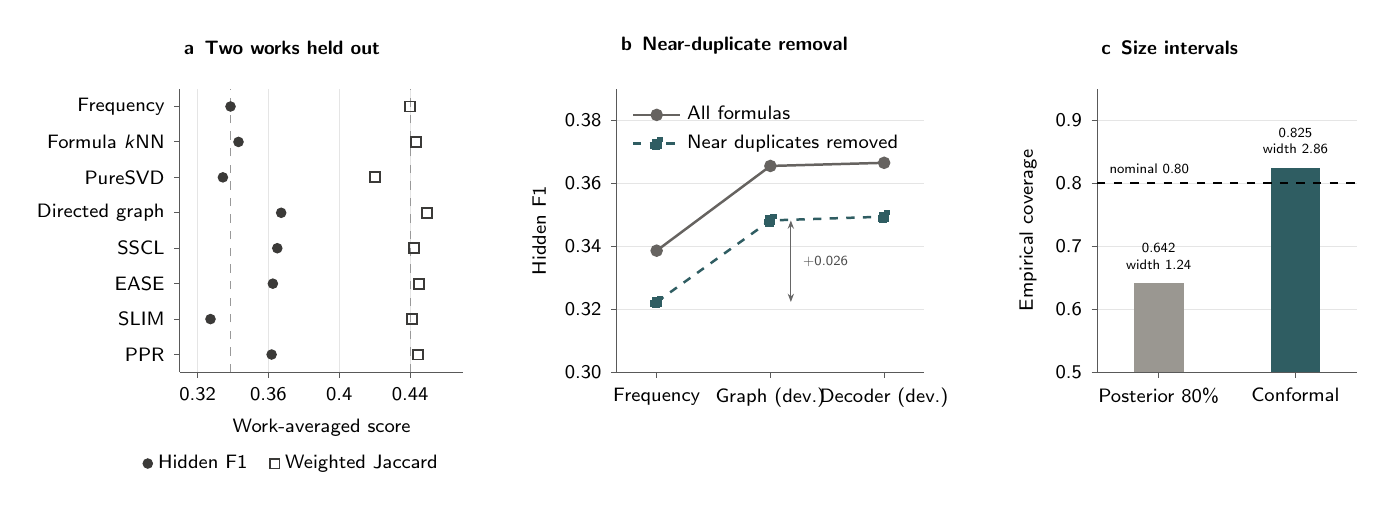
\begin{tikzpicture}
\begin{axis}[paper, at={(1.85cm,0)}, scale only axis, width=3.6cm, height=3.6cm,
  xmin=0.31, xmax=0.47, ymin=0.5, ymax=8.5, ytick={1,...,8},
  yticklabels={PPR,SLIM,EASE,SSCL,Directed graph,PureSVD,Formula $k$NN,Frequency},
  xtick={0.32,0.36,0.40,0.44}, xticklabel style={/pgf/number format/fixed,/pgf/number format/precision=2},
  xlabel={Work-averaged score}, xmajorgrids, title={\textbf{a}\enspace\textbf{Two works held out}},
  legend style={at={(0.4,-0.25)},anchor=north,legend columns=2,/tikz/every even column/.append style={column sep=6pt}}]
\draw[black!40,dashed] (axis cs:0.3386,0.5)--(axis cs:0.3386,8.5) (axis cs:0.4400,0.5)--(axis cs:0.4400,8.5);
\addplot[only marks,mark=*,mark size=1.7pt,color=cdark] coordinates {(0.3386,8) (0.3431,7) (0.3343,6) (0.3672,5) (0.3650,4) (0.3625,3) (0.3273,2) (0.3618,1)};
\addplot[only marks,mark=square,mark size=1.8pt,draw=cdark,line width=0.7pt] coordinates {(0.4400,8) (0.4435,7) (0.4200,6) (0.4494,5) (0.4423,4) (0.4450,3) (0.4408,2) (0.4445,1)};
\legend{Hidden F1,Weighted Jaccard}
\end{axis}
\begin{axis}[paper, at={(7.4cm,0)}, scale only axis, width=3.9cm, height=3.6cm,
  xmin=-0.35, xmax=2.35, ymin=0.30, ymax=0.39, xtick={0,1,2},
  xticklabels={Frequency,Graph (dev.),Decoder (dev.)}, ytick={0.30,0.32,0.34,0.36,0.38},
  yticklabel style={/pgf/number format/fixed,/pgf/number format/precision=2,/pgf/number format/fixed zerofill},
  ylabel={Hidden F1}, ymajorgrids, title={\textbf{b}\enspace\textbf{Near-duplicate removal}},
  legend style={at={(0.02,0.98)},anchor=north west,cells={anchor=west}}]
\addplot[color=cgray,mark=*,mark size=1.8pt,line width=0.9pt] coordinates {(0,0.3386) (1,0.3655) (2,0.3665)};
\addplot[color=cteal,mark=square*,mark size=1.8pt,line width=0.9pt,dashed] coordinates {(0,0.3223) (1,0.3482) (2,0.3494)};
\legend{All formulas,Near duplicates removed}
\draw[{Stealth[length=3pt]}-{Stealth[length=3pt]},black!60] (axis cs:1.18,0.3223)--(axis cs:1.18,0.3482);
\node[font=\sffamily\sansmath\tiny,text=black!70,anchor=west] at (axis cs:1.2,0.3352) {$+0.026$};
\end{axis}
\begin{axis}[paper, at={(13.5cm,0)}, scale only axis, width=3.3cm, height=3.6cm,
  ybar, bar width=18pt, ymin=0.5, ymax=0.95, symbolic x coords={Posterior,Conformal}, xtick={Posterior,Conformal}, enlarge x limits=0.45,
  xticklabels={Posterior 80\%,Conformal},
  ytick={0.5,0.6,0.7,0.8,0.9}, yticklabel style={/pgf/number format/fixed,/pgf/number format/precision=1,/pgf/number format/fixed zerofill},
  ylabel={Empirical coverage}, ymajorgrids, title={\textbf{c}\enspace\textbf{Size intervals}}]
\addplot[fill=clgray,draw=none,bar shift=0pt] coordinates {(Posterior,0.642)};
\addplot[fill=cteal,draw=none,bar shift=0pt] coordinates {(Conformal,0.825)};
\draw[black,dashed,line width=0.6pt] (rel axis cs:0,0.6667)--(rel axis cs:1,0.6667);
\node[font=\sffamily\sansmath\tiny,anchor=south west] at (rel axis cs:0.01,0.6667) {nominal 0.80};
\node[font=\sffamily\sansmath\tiny,align=center,anchor=south] at (axis cs:Posterior,0.648) {0.642\\width 1.24};
\node[font=\sffamily\sansmath\tiny,align=center,anchor=south] at (axis cs:Conformal,0.831) {0.825\\width 2.86};
\end{axis}
\end{tikzpicture}
\end{adjustwidth}
\caption{Secondary protocol (two held-out works). (\textbf{a}) Hidden F1 and weighted Jaccard for eight models (Table~\ref{tab:twowork}); dashed lines mark frequency. (\textbf{b}) Hidden F1 before and after removing nine formulas with a cross-work near duplicate, for frequency and the development-stage graph and decoder; the gain of the graph over frequency is preserved. (\textbf{c}) Empirical coverage and mean width of central 80\% size intervals before and after split-conformal expansion; the dashed line marks the nominal level.}
\label{fig:stress}
\end{figure}

\subsection{The Observation Mechanism Changes Difficulty More Than Ranking}
\label{sec:missing}

At 50\% observation, every structured model beat frequency under all four mechanisms (Table~\ref{tab:missing}). The differences among the structured models were small (at most 0.017), and the best model changed with the mechanism: the directed graph under abundance-biased retention, EASE under source-prefix retention, and SSCL under uniform retention and when $f$ was withheld. Given the resolution of six works, these differences in ordering should not be over-interpreted; the robust conclusion is that conditioning on observed materials helps under every mechanism tested.

\begin{table}[H]
\caption{Work-averaged hidden F1 under four observation mechanisms at 50\% observation.}
\label{tab:missing}
\small
\begin{tabularx}{\textwidth}{lCCCC}
\toprule
\textbf{Mechanism} & \textbf{Frequency} & \textbf{Directed graph} & \textbf{SSCL} & \textbf{EASE} \\
\midrule
Uniform & 0.378 & 0.426 & \textbf{0.426} & 0.423 \\
Abundance-biased & 0.389 & \textbf{0.430} & 0.426 & 0.429 \\
Source-list prefix & 0.399 & 0.468 & 0.466 & \textbf{0.481} \\
Uniform, $f$ withheld & 0.378 & 0.392 & \textbf{0.404} & 0.387 \\
\bottomrule
\end{tabularx}
\end{table}

The observed fraction changes the task itself (Figure~\ref{fig:missingness}). Under uniform, abundance-biased and $f$-withheld retention, hidden F1 falls as more of the formula is observed, because the hidden set shrinks to one or two materials that are disproportionately rare, and a single miss then costs a large share of F1. At 75\% uniform retention all models fell to about 0.27--0.29, and at 75\% abundance-biased retention frequency (0.355) matched or exceeded the structured models: once the principal ingredients are visible, what remains is a rare accent that no co-occurrence model predicts. Source-prefix retention behaves differently. Its curves are flat for SSCL (0.462 at 75\% versus 0.395 for frequency), consistent with base materials tending to be listed first, so that a prefix reveals the base from which the remaining materials can be inferred.

\begin{figure}[H]
\begin{adjustwidth}{-\extralength}{0cm}
\centering
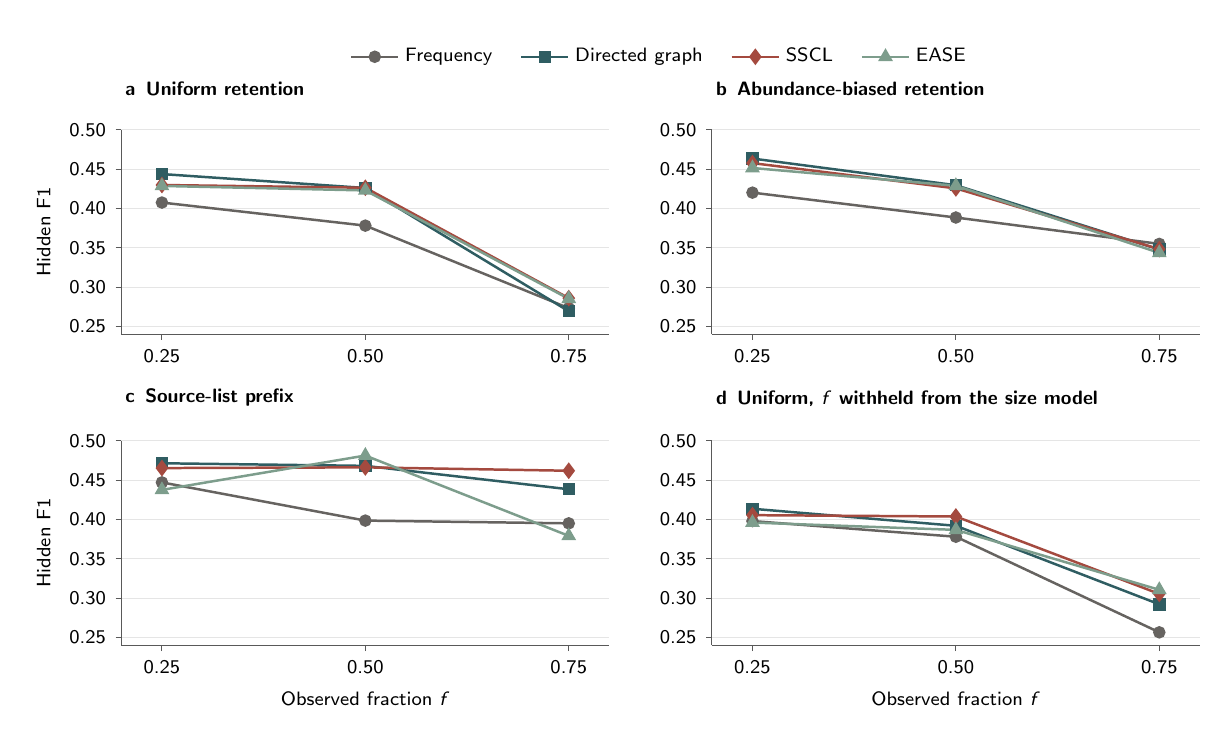
\begin{tikzpicture}
\begin{groupplot}[paper, group style={group size=2 by 2, horizontal sep=1.3cm, vertical sep=1.35cm,
     xlabels at=edge bottom, ylabels at=edge left},
  scale only axis, width=6.2cm, height=2.6cm, xmin=0.2, xmax=0.8, ymin=0.24, ymax=0.50,
  xtick={0.25,0.5,0.75}, xticklabels={0.25,0.50,0.75}, ytick={0.25,0.30,0.35,0.40,0.45,0.50},
  yticklabel style={/pgf/number format/fixed,/pgf/number format/precision=2,/pgf/number format/fixed zerofill},
  ymajorgrids, xlabel={Observed fraction $f$}, ylabel={Hidden F1},
  every axis plot/.append style={line width=0.9pt,mark size=1.8pt}]
\nextgroupplot[title={\textbf{a}\enspace\textbf{Uniform retention}},
  legend to name=fivelegend, legend columns=4, legend style={/tikz/every even column/.append style={column sep=8pt}}]
\addplot[color=cgray,mark=*] coordinates {(0.25,0.4075) (0.5,0.3782) (0.75,0.2734)};
\addplot[color=cteal,mark=square*] coordinates {(0.25,0.4437) (0.5,0.4260) (0.75,0.2695)};
\addplot[color=cred,mark=diamond*,mark size=2.3pt] coordinates {(0.25,0.4298) (0.5,0.4263) (0.75,0.2861)};
\addplot[color=csage,mark=triangle*,mark size=2.2pt] coordinates {(0.25,0.4286) (0.5,0.4229) (0.75,0.2853)};
\legend{Frequency,Directed graph,SSCL,EASE}
\nextgroupplot[title={\textbf{b}\enspace\textbf{Abundance-biased retention}}]
\addplot[color=cgray,mark=*] coordinates {(0.25,0.4201) (0.5,0.3885) (0.75,0.3550)};
\addplot[color=cteal,mark=square*] coordinates {(0.25,0.4634) (0.5,0.4295) (0.75,0.3478)};
\addplot[color=cred,mark=diamond*,mark size=2.3pt] coordinates {(0.25,0.4576) (0.5,0.4255) (0.75,0.3484)};
\addplot[color=csage,mark=triangle*,mark size=2.2pt] coordinates {(0.25,0.4514) (0.5,0.4288) (0.75,0.3436)};
\nextgroupplot[title={\textbf{c}\enspace\textbf{Source-list prefix}}]
\addplot[color=cgray,mark=*] coordinates {(0.25,0.4471) (0.5,0.3986) (0.75,0.3951)};
\addplot[color=cteal,mark=square*] coordinates {(0.25,0.4714) (0.5,0.4681) (0.75,0.4384)};
\addplot[color=cred,mark=diamond*,mark size=2.3pt] coordinates {(0.25,0.4653) (0.5,0.4662) (0.75,0.4619)};
\addplot[color=csage,mark=triangle*,mark size=2.2pt] coordinates {(0.25,0.4376) (0.5,0.4812) (0.75,0.3792)};
\nextgroupplot[title={\textbf{d}\enspace\textbf{Uniform, $f$ withheld from the size model}}]
\addplot[color=cgray,mark=*] coordinates {(0.25,0.3980) (0.5,0.3781) (0.75,0.2567)};
\addplot[color=cteal,mark=square*] coordinates {(0.25,0.4136) (0.5,0.3920) (0.75,0.2923)};
\addplot[color=cred,mark=diamond*,mark size=2.3pt] coordinates {(0.25,0.4055) (0.5,0.4038) (0.75,0.3055)};
\addplot[color=csage,mark=triangle*,mark size=2.2pt] coordinates {(0.25,0.3961) (0.5,0.3868) (0.75,0.3107)};
\end{groupplot}
\node[anchor=south] at ($(group c1r1.north)!0.5!(group c2r1.north)+(0,0.55cm)$) {\pgfplotslegendfromname{fivelegend}};
\end{tikzpicture}
\end{adjustwidth}
\caption{Hidden F1 as a function of the observed fraction under four observation mechanisms. (\textbf{a}) Uniform retention. (\textbf{b}) Retention probability proportional to reference mass. (\textbf{c}) The first materials in source order. (\textbf{d}) Uniform retention with $f$ withheld from the size model. Points are work-averaged means over the six outer folds of the primary protocol; shared axes show changes in both difficulty and ordering.}
\label{fig:missingness}
\end{figure}

\subsection{Calibrated Probabilities and Size Intervals}
\label{sec:uncertainty}

Raw SSCL scores were overconfident: the 186 candidates scored above 0.8 had a mean score of 0.839 but were present only 60.8\% of the time (Table~\ref{tab:calib}, Figure~\ref{fig:calibration}). Temperature scaling lowered every error metric but sharpened the scores, so that 455 candidates exceeded 0.8 with an empirical frequency of only 0.527. This is the expected failure of a map that can only rescale log-odds about zero. The two-parameter logistic map, which can also shift them, reduced the Brier score from 0.0427 to 0.0340, NLL from 0.1572 to 0.1262 and ACE from 0.0579 to 0.0145, and left only two scores above 0.8. For users, a calibrated score has a concrete meaning: among candidates scored $p$ in books not used for fitting, a fraction of about $p$ belongs to the formula.

\begin{table}[H]
\caption{Nested calibration of SSCL candidate scores (work-averaged). The last three columns describe predictions with $p>0.8$.}
\label{tab:calib}
\small
\begin{tabularx}{\textwidth}{lCCCCCC}
\toprule
\textbf{Method} & \textbf{Brier} & \textbf{NLL} & \textbf{ACE} & \textbf{Count} & \textbf{Mean $\bm p$} & \textbf{Observed rate} \\
\midrule
Uncalibrated & 0.0427 & 0.1572 & 0.0579 & 186 & 0.839 & 0.608 \\
Temperature & 0.0406 & 0.1456 & 0.0371 & 455 & 0.874 & 0.527 \\
Logistic & \textbf{0.0340} & \textbf{0.1262} & \textbf{0.0145} & 2 & 0.831 & 1.000 \\
\bottomrule
\end{tabularx}
\end{table}

\begin{figure}[H]
\begin{adjustwidth}{-\extralength}{0cm}
\centering
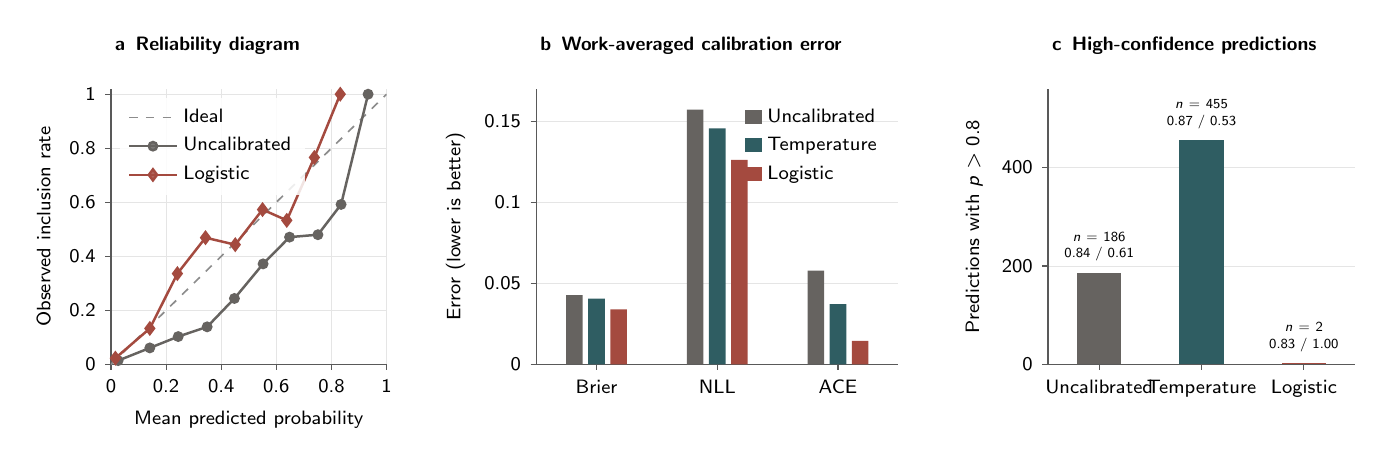
\begin{tikzpicture}
\begin{axis}[paper, at={(0.9cm,0)}, scale only axis, width=3.5cm, height=3.5cm,
  xmin=0, xmax=1, ymin=0, ymax=1.02, xtick={0,0.2,0.4,0.6,0.8,1}, ytick={0,0.2,0.4,0.6,0.8,1},
  xticklabel style={/pgf/number format/fixed}, yticklabel style={/pgf/number format/fixed},
  xlabel={Mean predicted probability}, ylabel={Observed inclusion rate}, grid=major,
  title={\textbf{a}\enspace\textbf{Reliability diagram}},
  legend style={at={(0.03,0.97)},anchor=north west,cells={anchor=west},fill=white,fill opacity=0.85,text opacity=1}]
\addplot[black!45,dashed,line width=0.6pt] coordinates {(0,0) (1,1)};
\addplot[color=cgray,mark=*,mark size=1.5pt,line width=0.9pt] coordinates {(0.026,0.014) (0.141,0.061) (0.244,0.103) (0.349,0.139) (0.448,0.244) (0.552,0.372) (0.648,0.471) (0.751,0.480) (0.835,0.592) (0.933,1.000)};
\addplot[color=cred,mark=diamond*,mark size=2pt,line width=0.9pt] coordinates {(0.016,0.023) (0.141,0.133) (0.241,0.336) (0.343,0.469) (0.451,0.443) (0.550,0.573) (0.638,0.533) (0.738,0.766) (0.832,1.000)};
\legend{Ideal,Uncalibrated,Logistic}
\end{axis}
\begin{axis}[paper, at={(6.3cm,0)}, scale only axis, width=4.6cm, height=3.5cm,
  ybar, bar width=6pt, ymin=0, ymax=0.17, symbolic x coords={Brier,NLL,ACE}, xtick=data, enlarge x limits=0.25,
  yticklabel style={/pgf/number format/fixed,/pgf/number format/precision=2}, ylabel={Error (lower is better)}, ymajorgrids,
  title={\textbf{b}\enspace\textbf{Work-averaged calibration error}},
  legend style={at={(0.98,0.97)},anchor=north east,cells={anchor=west}}, legend image code/.code={\draw[#1,draw=none] (0cm,-0.08cm) rectangle (0.22cm,0.1cm);}]
\addplot[fill=cgray,draw=none] coordinates {(Brier,0.0427) (NLL,0.1572) (ACE,0.0579)};
\addplot[fill=cteal,draw=none] coordinates {(Brier,0.0406) (NLL,0.1456) (ACE,0.0371)};
\addplot[fill=cred,draw=none] coordinates {(Brier,0.0340) (NLL,0.1262) (ACE,0.0145)};
\legend{Uncalibrated,Temperature,Logistic}
\end{axis}
\begin{axis}[paper, at={(12.8cm,0)}, scale only axis, width=3.9cm, height=3.5cm,
  ybar, bar width=16pt, ymin=0, ymax=560, symbolic x coords={Uncalibrated,Temperature,Logistic}, xtick={Uncalibrated,Temperature,Logistic}, enlarge x limits=0.25,
  ylabel={Predictions with $p>0.8$}, ymajorgrids, title={\textbf{c}\enspace\textbf{High-confidence predictions}}]
\addplot[fill=cgray,draw=none,bar shift=0pt] coordinates {(Uncalibrated,186)};
\addplot[fill=cteal,draw=none,bar shift=0pt] coordinates {(Temperature,455)};
\addplot[fill=cred,draw=none,bar shift=0pt] coordinates {(Logistic,2)};
\node[font=\sffamily\sansmath\tiny,align=center,anchor=south] at (axis cs:Uncalibrated,190) {$n=186$\\0.84 / 0.61};
\node[font=\sffamily\sansmath\tiny,align=center,anchor=south] at (axis cs:Temperature,459) {$n=455$\\0.87 / 0.53};
\node[font=\sffamily\sansmath\tiny,align=center,anchor=south] at (axis cs:Logistic,6) {$n=2$\\0.83 / 1.00};
\end{axis}
\end{tikzpicture}
\end{adjustwidth}
\caption{Nested probability calibration of SSCL scores. (\textbf{a}) Pooled reliability diagram before and after logistic calibration. (\textbf{b}) Work-averaged Brier score, negative log-likelihood and adaptive calibration error. (\textbf{c}) Number of predictions above 0.8, labelled with mean probability/empirical frequency. The two logistic-calibrated predictions above 0.8 are too few for a stable estimate.}
\label{fig:calibration}
\end{figure}

For formula size, the central 80\% posterior interval covered the true size in only 64.2\% of 1660 instances of the secondary protocol (mean width 1.24 materials), because the posterior ignores between-book variation in formula length. Split-conformal expansion, calibrated on 420 development instances ($\lceil 421\times0.8\rceil/420=0.8024$), widened every interval by one material and raised coverage to 82.5\% at a mean width of 2.86 (Figure~\ref{fig:stress}c). The finite-sample guarantee of conformal prediction assumes exchangeability of calibration and test instances, which work-blocked data satisfy only approximately; the empirical coverage is nevertheless close to nominal.

\subsection{Where the Errors Come From}
\label{sec:errors}

\paragraph{Rarity.} The secondary protocol contains 6450 hidden-material opportunities pooled over folds and masks (Table~\ref{tab:rarity}). Their recall decomposes as a weighted average over frequency strata, $R=\sum_k\varpi_kR_k$, where $\varpi_k$ is the share of opportunities in stratum $k$. Materials seen in at least five training formulas account for 60.1\% of opportunities and 97.7\% of all recovered materials (recall 0.573). Recall collapses to 0.056 for materials seen two to four times and 0.023 for materials seen once. Materials absent from the training vocabulary make up 22.4\% of opportunities and can never be predicted, so the recall of any ranking model is bounded by $1-0.224=0.776$ in this protocol. Rarity explains more error than formula size: formulas with at least eight materials reached hidden F1 0.446, compared with 0.352 for two to four materials and 0.344 for five to seven.

\begin{table}[H]
\caption{Hidden-material recall by training frequency (secondary protocol, pooled over folds and masks; used for error localisation, not inference).}
\label{tab:rarity}
\small
\begin{tabularx}{\textwidth}{lCCCC}
\toprule
\textbf{Training frequency} & \textbf{Opportunities} & \textbf{Share} & \textbf{Recovered} & \textbf{Recall} \\
\midrule
Absent from vocabulary & 1445 & 0.224 & 0 & 0.000 \\
One formula & 342 & 0.053 & 8 & 0.023 \\
Two to four formulas & 787 & 0.122 & 44 & 0.056 \\
At least five formulas & 3876 & 0.601 & 2221 & 0.573 \\
\midrule
All & 6450 & 1.000 & 2273 & 0.352 \\
\bottomrule
\end{tabularx}
\end{table}

False positives concentrate on the hubs of the co-formulation graph: white sandalwood (462 false additions), borneol (409), musk (378) and generic agarwood (376). Frequent false negatives include scrophularia root, spikenard, Zhan-grade agarwood, frankincense and clove. The model learns productive hubs and over-uses them when a target book follows a different convention.

\paragraph{A worked example.} The selected case is the Hong \emph{yinxiang} formula introduced in Section~\ref{sec:intro} (Table~\ref{tab:case}). With six of eleven materials observed, the model predicted the correct size and recovered three of five hidden materials (Zhan-grade agarwood, borneol and white sandalwood), missed frankincense and licorice, and added clove and \emph{linglingxiang}; precision, recall and F1 all equal 0.60. Proportions were less accurate than identities: Zhan-grade agarwood received 0.117 of the mass against 0.332 in the source, and borneol 0.099 against 0.013. The weighted Jaccard is 0.483; by Lemma~\ref{lem:wj} the observed 45.3\% of the mass alone guarantees at least $0.453/1.547=0.293$. The hidden-mass score is $1-\TV/m_i=0.36$: of the 54.7\% of the mass that was hidden, the prediction placed about a third on the correct materials.

\begin{table}[H]
\caption{Completion of the Hong \emph{yinxiang} formula (mask seed 17). Observed materials keep their reference fractions; a dash marks a material that is absent from the reference or from the prediction. Reference fractions are rounded and sum to 0.996.}
\label{tab:case}
\small
\begin{tabularx}{\textwidth}{LlCC}
\toprule
\textbf{Material} & \textbf{Outcome} & \textbf{Reference} & \textbf{Predicted} \\
\midrule
Agarwood & observed & 0.066 & 0.066 \\
Aromatic grass & observed & 0.266 & 0.266 \\
Musk & observed & 0.053 & 0.053 \\
Onycha & observed & 0.001 & 0.001 \\
Patchouli & observed & 0.001 & 0.001 \\
Spikenard & observed & 0.066 & 0.066 \\
Zhan-grade agarwood & recovered & 0.332 & 0.117 \\
Borneol & recovered & 0.013 & 0.099 \\
White sandalwood & recovered & 0.066 & 0.103 \\
Frankincense & missed & 0.066 & --- \\
Licorice & missed & 0.066 & --- \\
Clove & falsely added & --- & 0.106 \\
\emph{Linglingxiang} & falsely added & --- & 0.120 \\
\bottomrule
\end{tabularx}
\end{table}

\paragraph{Composition rule.} Lemma~\ref{lem:wj} also explains a development result. Replacing an unconstrained composition decoder by rule~\eqref{eq:composition}, which keeps the observed fractions and closes the prediction to the residual mass, raised weighted Jaccard in the secondary protocol from 0.387 to 0.427 without changing a single selected material. Part of this gain is the guaranteed floor that the rule enforces, which is why we recommend reporting $1-\TV_i/m_i$ alongside weighted Jaccard.

\paragraph{Chemistry.} A chemical-similarity kernel built from specimen-level analytical profiles of 18 materials neither helped nor hurt completion (hidden F1 0.3905 with the kernel, 0.3911 without; Appendix~\ref{app:dev}). The 18 profiled materials represent only 22.2\% of material types but 65.2\% of aromatic mentions in the ratio-ready corpus, so the null result plausibly concerns common materials whose co-formulation is already well estimated from the texts.

%=================================================================
\section{Discussion}
\label{sec:discussion}

\subsection{What Transfers Between Books}
Across six held-out books, knowing part of a formula improves the prediction of the rest by about 0.05 in F1, roughly a 13\% relative improvement over frequency, and the improvement appeared in every book where the methods differed. It survives holding out two books at once, removal of near duplicates and four observation mechanisms. The directed graph, SSCL, EASE and PPR all capture it, whereas formula-level nearest neighbours and low-rank factorisation largely do not. The transferable object is therefore the pairwise conditional structure of co-formulation: which materials habitually accompany which, independently of the compiler. It is consistent with the common description of incense formulas as a base of woods and resins completed by characteristic accents, and it gives heritage scholars a quantitative way to flag likely lacunae in damaged or abridged witnesses.

\subsection{Why the Heterogeneity Penalty Is Inert}
\label{sec:disc-penalty}
SSCL was designed to prefer associations that hold across books. It matched but did not beat the directed graph, and the 90\% interval limits the penalty's effect to about $\pm0.01$ F1. Three observations explain this. First, by Remark~\ref{rem:dispersion}, $s_{ab}$ is estimated from at most five training works (four in inner folds), so its relative error is of order 35--40\%, and the ranking perturbation it induces is largely noise. Second, the edges that matter for recall are those between common materials (Table~\ref{tab:rarity}), and these are estimated precisely and consistently in every book, leaving little heterogeneity to penalise. Third, the edges that are genuinely book-specific involve rare materials that neither model recovers. Proposition~\ref{prop:robust} suggests when SSCL should help: with more source domains, $s_{ab}$ becomes informative, and the lower-quantile interpretation offers a principled choice of $\gamma$ through the desired predictive level. The penalty is therefore a hypothesis to retest as the corpus grows rather than a component to discard.

\subsection{Scale and Quality Are Separate Variables}
Weak records helped the quantity that depends on counts (formula size) and did not help the quantity that depends on identities (ingredient edges). An erroneous material identity or a merged formula boundary adds spurious pairs to many edges at once, whereas a slightly wrong record still contributes a correct size. The practical implication is that review effort, not extraction volume, limits ingredient recovery. Because inner validation chose $\eta>0$ in five of six folds, the weak pool contains useful structure. It should be reviewed in order of expected information gain: families that introduce a material that is rare or absent in some fold (Table~\ref{tab:rarity}), families that bridge collections, and families that provide a second observation of a high-dispersion edge.

\subsection{Lessons for Evaluating Historical Reconstruction}
Three design choices changed conclusions and should be standard. Blocking by work and by collection measures transfer to a new book rather than memorisation of a known one. Reporting the observation mechanism is necessary because the observed fraction and mechanism change task difficulty more than they change model ranking. Composition scores need a reference point: by Lemma~\ref{lem:wj}, weighted Jaccard contains a floor determined by the observed mass, and the hidden-mass score $1-\TV/m$ removes it. Finally, the number of books, not the number of formulas, governs statistical precision. With six works and one tie, no test can reach $p<0.0625$ (Proposition~\ref{prop:floor}); reporting randomisation intervals and leave-one-work-out ranges conveys the evidence more faithfully than a binary significance verdict.

\subsection{Limitations}
The gold set was reviewed by a single curator, so inter-annotator agreement on formula boundaries, material identities and quantities is not yet available. The six work groups are unequal in size, and two contain two and six formulas; conclusions about individual books, particularly Xiaolu, are correspondingly weak. Observation mechanisms were simulated; empirical damage patterns from parallel witnesses would provide more realistic masks. The near-duplicate analysis, the composition-rule comparison and the chemistry ablation used development-stage configurations (Appendix~\ref{app:dev}) rather than the final tuned models, and are reported as supporting evidence only. Finally, canonical material identities for historical names are themselves uncertain for part of the vocabulary; the recall ceiling in Table~\ref{tab:rarity} partly reflects this uncertainty.

\subsection{Future Work}
Four extensions follow directly. (i) Reviewing the 146 weak records and adding further public-domain incense collections would increase both the gold set and, more importantly, the number of work domains, which is what limits inference and the usefulness of the SSCL penalty. (ii) A second independent annotation of a stratified sample would quantify label reliability and support a probabilistic label model for the weak pool~\cite{ratner2017}. (iii) Parallel witnesses can be aligned to learn an empirical deletion model $p(O_i\mid S_i,d_i)$ to replace simulated masks. (iv) Proportions should be modelled on the simplex, for example by logistic-normal or Dirichlet regression~\cite{aitchison1982} with the co-formulation graph as a structured prior, and chemical information should enter through directed interaction features relevant to combustion rather than symmetric similarity.

%=================================================================
\section{Conclusions}
\label{sec:conclusions}

Restoring fragmentary historical incense formulas can be posed as weighted set completion under source shift and evaluated honestly by holding out whole books. On a provenance-indexed corpus with 91 reviewed formulas from six work groups, conditional co-formulation structure transfers between books and improves hidden-ingredient F1 from 0.378 to 0.426 over global frequency, consistently across works. A source-stable variant with a robust-optimisation interpretation matches but does not improve on the plain directed graph at six domains. Unreviewed records improve size prediction but not ingredient identification, nested calibration makes graph scores interpretable as probabilities, and material rarity sets the main remaining limit. The benchmark, its evidence hierarchy and its inference conventions are intended as a reusable basis for quantitative reconstruction of historical recipes.

%=================================================================
\vspace{6pt}

\authorcontributions{Conceptualization, H.Z.; methodology, H.Z.; software, H.Z.; validation, H.Z.; formal analysis, H.Z.; investigation, H.Z.; data curation, H.Z.; writing---original draft preparation, H.Z.; writing---review and editing, H.Z.; visualization, H.Z. The author has read and agreed to the published version of the manuscript.}

% TODO(author): confirm funding.
\funding{This research received no external funding.}

\institutionalreview{Not applicable. The study analyses public historical texts and published chemical records.}

\informedconsent{Not applicable.}

% TODO(author): insert the repository DOI before submission.
\dataavailability{The curated formula records, source locators, material ontology, deterministic split and mask definitions, experiment configurations, model code, tests and the source data for all figures and tables are available at [repository DOI to be inserted]. Records retain the source attribution and rights statement of each transcription.}

% TODO(author): MDPI requires disclosure of generative-AI assistance; adapt this sentence to the actual use.
\acknowledgments{During the preparation of this manuscript, the author used generative AI tools to assist with drafting and editing the text and figures. The author reviewed and edited all output and takes full responsibility for the content of this publication.}

\conflictsofinterest{The author declares no conflicts of interest.}

\abbreviations{Abbreviations}{
The following abbreviations are used in this manuscript:\\

\noindent
\begin{tabular}{@{}ll}
ACE & Adaptive calibration error\\
EASE & Embarrassingly shallow autoencoder\\
LOWO & Leave one work out\\
MAE & Mean absolute error\\
NLL & Negative log-likelihood\\
PPR & Personalised PageRank\\
SLIM & Sparse linear method\\
SSCL & Source-stable conditional lift\\
TV & Total variation
\end{tabular}
}

%=================================================================
\appendixtitles{yes}
\appendixstart
\appendix
\section[\appendixname~\thesection]{Development-Stage Analyses}
\label{app:dev}

\paragraph{Probabilistic decoder.} Before the final graph models were tuned, a probabilistic decoder was developed that scores each candidate with a logistic model on graph-derived features and averages predictions over 200 posterior parameter draws. It is not part of the main comparison. It served as the host model for the chemistry ablation, appears as ``decoder (dev.)'' in the near-duplicate test (Figure~\ref{fig:stress}b), and was used for the composition-rule comparison in Section~\ref{sec:errors}.

\paragraph{Chemical similarity.} A chemical registry links 18 of the 81 canonical materials to specimen-level analytical profiles drawn from 17 publications and 40 PubChem compounds, covering, among others, agarwood, sandalwood, frankincense, clove, cassia and cyperus~\cite{ngan2020,fatima2019,distefano2020,benhassine2021,firmino2018,hu2017}. Profiles record taxon, plant part, preparation, analytical method and measurement basis; peak-area data, calibrated concentrations and presence-only reports are kept as separate evidence types. For compound sets $\mathcal P_a,\mathcal P_b$ with Morgan fingerprint bit sets $B_u$~\cite{rogers2010}, the fingerprint similarity is $T_{ab}=\max_{u\in\mathcal P_a,v\in\mathcal P_b}|B_u\cap B_v|/|B_u\cup B_v|$. Physicochemical vectors (molecular weight, hydrogen-bond donors and acceptors, rotatable bonds, topological polar surface area, log$P$) and controlled odour-tag vectors (woody, balsamic, spicy, floral, camphoraceous, animalic and others) are abundance-weighted where abundances are available, and compared by cosine similarity. The kernel
\begin{equation}
\mathcal K_{ab}=\omega_fT_{ab}+\omega_x\max\bigl(0,C^{\mathrm{phys}}_{ab}\bigr)+\omega_o\max\bigl(0,C^{\mathrm{odor}}_{ab}\bigr),\qquad \omega_f+\omega_x+\omega_o=1,
\label{eq:kernel}
\end{equation}
was added to the decoder for the 18 covered materials. Table~\ref{tab:chem} reports the ablation and an inverse-odour task in which 44 formulas are reconstructed from their odour-tag profile.

\begin{table}[H]
\caption{Chemistry ablations (development stage). Completion reports hidden F1; inverse odour reports weighted Jaccard on 44 formulas.}
\label{tab:chem}
\small
\begin{tabularx}{\textwidth}{lLc}
\toprule
\textbf{Task} & \textbf{Model} & \textbf{Score} \\
\midrule
Completion & Decoder without chemistry & 0.3911 \\
Completion & Decoder with chemical kernel & 0.3905 \\
Inverse odour & Odour-profile $k$NN & 0.2913 \\
Inverse odour & Forward-consistent decoder & 0.2824 \\
Inverse odour & Decoder without chemistry & 0.2835 \\
Inverse odour & Shuffled chemical profiles & 0.2863 \\
\bottomrule
\end{tabularx}
\end{table}

\paragraph{Computational profile.} Dense graph construction costs $O(NM^2)$, or $O(N\bar K^2)$ when pairs are accumulated sparsely; scoring one query costs $O(|O_i|M)$ plus $O(M)$ expected time for top-$K$ selection. The implementation uses NumPy and scikit-learn~\cite{pedregosa2011} with dense arrays ($M\le81$). On one Apple arm64 process with data loaded, the development decoder, which is more expensive than the graph models, fitted 85 formulas and 80 materials in a median 0.115 s (interquartile range 0.005 s, 11 runs), and one prediction with 200 posterior draws took a median 1.70 ms (interquartile range 0.14 ms). The graph models avoid optimisation and sampling and are faster still.

\section[\appendixname~\thesection]{Notation}
\label{app:notation}

\begin{table}[H]
\caption{Principal notation.}
\label{tab:notation}
\small
\begin{tabularx}{\textwidth}{lL}
\toprule
\textbf{Symbol} & \textbf{Meaning} \\
\midrule
$i$; $a,b$; $d$ & formula; observed and candidate materials; work group \\
$S_i,O_i,H_i$; $K_i$ & complete, observed and hidden material sets; formula size \\
$q_{ij},w_{ij}$; $m_i$ & converted mass and closed fraction; residual (hidden) mass \\
$f$; $o(K,f)$ & requested observed fraction; number of observed materials \\
$\pi_b,\pi_{bd}$ & global and work-specific smoothed prevalence \\
$G_{ab}$ & directed conditional edge \\
$\bar\theta_{abd},\ell_{abd},v_{ad}$ & within-work conditional, lift and exposure weight \\
$\mu_{ab},s_{ab}$; $G^\star_{ab},G^{\mathrm{SS}}_{ab}$ & pooled lift and dispersion; robust and blended SSCL edges \\
$\alpha,\kappa,\gamma,\lambda$ & smoothing, work shrinkage, dispersion penalty, blend weight \\
$z_i,\fmly(i),C(i)$; $\omega_i,\eta$ & evidence class, family, collection; record weight, weak-label weight \\
$\mathcal W_{d^\star}$ & admissible weak pool for test work $d^\star$ \\
$p_{ib}$; $\widehat K_i,\widehat H_i,\widehat{\bm w}_i$ & candidate score; predicted size, hidden set and composition \\
$\Delta_{md}$; $D$ & work-level difference from frequency; number of works \\
\bottomrule
\end{tabularx}
\end{table}

%=================================================================
\begin{adjustwidth}{-\extralength}{0cm}
\reftitle{References}
\begin{thebibliography}{999}

\bibitem{bembibre2017} Bembibre, C.; Strli\v{c}, M. Smell of heritage: A framework for the identification, analysis and archival of historic odours. \emph{Herit. Sci.} \textbf{2017}, \emph{5}, 2. \url{https://doi.org/10.1186/s40494-016-0114-1}.

\bibitem{lisena2022} Lisena, P.; Schwabe, D.; van Erp, M.; Troncy, R.; Tullett, W.; Leemans, I.; Marx, L.; Ehrich, S.C. Capturing the semantics of smell: The Odeuropa data model for olfactory heritage information. In \emph{The Semantic Web. ESWC 2022}; Springer: Cham, Switzerland, 2022; pp. 387--405. \url{https://doi.org/10.1007/978-3-031-06981-9_23}.

\bibitem{paolin2026} Paolin, E.; Di Gianvincenzo, F.; Torres-Elguera, J.C.; Ram\v{s}ak, M.; Kralj Cigi\'{c}, I.; Sawoszczuk, T.; Strli\v{c}, M. A systematic approach to the scientific reproduction of historical smells: Case study of a 20th-century perfume flask. \emph{npj Herit. Sci.} \textbf{2026}. \url{https://doi.org/10.1038/s40494-026-02699-x}.

\bibitem{keller2017} Keller, A.; Gerkin, R.C.; Guan, Y.; Dhurandhar, A.; Turu, G.; Szalai, B.; Mainland, J.D.; Ihara, Y.; Yu, C.W.; Wolfinger, R.; et~al. Predicting human olfactory perception from chemical features of odor molecules. \emph{Science} \textbf{2017}, \emph{355}, 820--826. \url{https://doi.org/10.1126/science.aal2014}.

\bibitem{gutierrez2018} Guti\'{e}rrez, E.D.; Dhurandhar, A.; Keller, A.; Meyer, P.; Cecchi, G.A. Predicting natural language descriptions of mono-molecular odorants. \emph{Nat. Commun.} \textbf{2018}, \emph{9}, 4979. \url{https://doi.org/10.1038/s41467-018-07439-9}.

\bibitem{lee2023} Lee, B.K.; Mayhew, E.J.; Sanchez-Lengeling, B.; Wei, J.N.; Qian, W.W.; Little, K.A.; Andres, M.; Nguyen, B.B.; Moloy, T.; Yasonik, J.; et~al. A principal odor map unifies diverse tasks in olfactory perception. \emph{Science} \textbf{2023}, \emph{381}, 999--1006. \url{https://doi.org/10.1126/science.ade4401}.

\bibitem{debnath2021} Debnath, T.; Prasetyawan, D.; Nakamoto, T. Predicting odor perception of mixed scent from mass spectrometry. \emph{J. Electrochem. Soc.} \textbf{2021}, \emph{168}, 117505. \url{https://doi.org/10.1149/1945-7111/ac33e0}.

\bibitem{hamel2024} Hamel, E.A.; Castro, J.B.; Gould, T.J.; Pellegrino, R.; Liang, Z.; Coleman, L.A.; Patel, F.; Wallace, D.S.; Bhatnagar, T.; Mainland, J.D.; et~al. Pyrfume: A window to the world's olfactory data. \emph{Sci. Data} \textbf{2024}, \emph{11}, 1220. \url{https://doi.org/10.1038/s41597-024-04051-z}.

\bibitem{sisson2025} Sisson, L.; Barsainyan, A.A.; Sharma, M.; Kumar, R. Deep learning for odor prediction on aroma-chemical blends. \emph{ACS Omega} \textbf{2025}, \emph{10}, 8980--8992. \url{https://doi.org/10.1021/acsomega.4c07078}.

\bibitem{thomasdanguin2014} Thomas-Danguin, T.; Sinding, C.; Romagny, S.; El~Mountassir, F.; Atanasova, B.; Le~Berre, E.; Le~Bon, A.M.; Coureaud, G. The perception of odor objects in everyday life: A review on the processing of odor mixtures. \emph{Front. Psychol.} \textbf{2014}, \emph{5}, 504. \url{https://doi.org/10.3389/fpsyg.2014.00504}.

\bibitem{aleixandre2024} Aleixandre, M.; Prasetyawan, D.; Nakamoto, T. Automatic scent creation by cheminformatics method. \emph{Sci. Rep.} \textbf{2024}, \emph{14}, 31284. \url{https://doi.org/10.1038/s41598-024-82654-7}.

\bibitem{steck2019} Steck, H. Embarrassingly shallow autoencoders for sparse data. In Proceedings of the World Wide Web Conference, San Francisco, CA, USA, 13--17 May 2019; pp. 3251--3257. \url{https://doi.org/10.1145/3308558.3313710}.

\bibitem{ning2011} Ning, X.; Karypis, G. SLIM: Sparse linear methods for top-N recommender systems. In Proceedings of the 2011 IEEE 11th International Conference on Data Mining, Vancouver, BC, Canada, 11--14 December 2011; pp. 497--506. \url{https://doi.org/10.1109/ICDM.2011.134}.

\bibitem{cremonesi2010} Cremonesi, P.; Koren, Y.; Turrin, R. Performance of recommender algorithms on top-N recommendation tasks. In Proceedings of the Fourth ACM Conference on Recommender Systems, Barcelona, Spain, 26--30 September 2010; pp. 39--46. \url{https://doi.org/10.1145/1864708.1864721}.

\bibitem{wu2015} Wu, B.; Lyu, S.; Ghanem, B. ML-MG: Multi-label learning with missing labels using a mixed graph. In Proceedings of the IEEE International Conference on Computer Vision, Santiago, Chile, 7--13 December 2015; pp. 4157--4165. \url{https://doi.org/10.1109/ICCV.2015.473}.

\bibitem{zhao2018} Zhao, H.; Rai, P.; Du, L.; Buntine, W. Bayesian multi-label learning with sparse features and labels, and label co-occurrences. In Proceedings of the 21st International Conference on Artificial Intelligence and Statistics, Playa Blanca, Spain, 9--11 April 2018; PMLR~84, pp. 1943--1951.

\bibitem{ratner2017} Ratner, A.; Bach, S.H.; Ehrenberg, H.; Fries, J.; Wu, S.; R\'{e}, C. Snorkel: Rapid training data creation with weak supervision. \emph{Proc. VLDB Endow.} \textbf{2017}, \emph{11}, 269--282. \url{https://doi.org/10.14778/3157794.3157797}.

\bibitem{sorbi2026} Sorbi, M.; Moccozet, L.; Marchand-Maillet, S. Weakly supervised named entity recognition for historical texts. In Proceedings of the 10th Joint SIGHUM Workshop on Computational Linguistics for Cultural Heritage, Social Sciences, Humanities and Literature (LaTeCH-CLfL 2026); Association for Computational Linguistics, 2026. \url{https://aclanthology.org/2026.latechclfl-1.6/}.

\bibitem{goel2024} Goel, M.; Agarwal, A.; Agrawal, S.; Kapuriya, J.; Konam, A.V.; Gupta, R.; Rastogi, S.; Niharika; Bagler, G. Deep learning based named entity recognition models for recipes. In Proceedings of the 2024 Joint International Conference on Computational Linguistics, Language Resources and Evaluation (LREC-COLING 2024), Torino, Italy, 20--25 May 2024; pp. 4542--4554.

\bibitem{aitchison1982} Aitchison, J. The statistical analysis of compositional data. \emph{J. R. Stat. Soc. Ser. B} \textbf{1982}, \emph{44}, 139--160. \url{https://doi.org/10.1111/j.2517-6161.1982.tb01195.x}.

\bibitem{rubin1976} Rubin, D.B. Inference and missing data. \emph{Biometrika} \textbf{1976}, \emph{63}, 581--592. \url{https://doi.org/10.1093/biomet/63.3.581}.

\bibitem{bental2009} Ben-Tal, A.; El~Ghaoui, L.; Nemirovski, A. \emph{Robust Optimization}; Princeton University Press: Princeton, NJ, USA, 2009.

\bibitem{dersimonian1986} DerSimonian, R.; Laird, N. Meta-analysis in clinical trials. \emph{Control. Clin. Trials} \textbf{1986}, \emph{7}, 177--188. \url{https://doi.org/10.1016/0197-2456(86)90046-2}.

\bibitem{page1999} Page, L.; Brin, S.; Motwani, R.; Winograd, T. \emph{The PageRank Citation Ranking: Bringing Order to the Web}; Technical Report; Stanford InfoLab: Stanford, CA, USA, 1999.

\bibitem{cover1967} Cover, T.M.; Hart, P.E. Nearest neighbor pattern classification. \emph{IEEE Trans. Inf. Theory} \textbf{1967}, \emph{13}, 21--27. \url{https://doi.org/10.1109/TIT.1967.1053964}.

\bibitem{lei2018} Lei, J.; G'Sell, M.; Rinaldo, A.; Tibshirani, R.J.; Wasserman, L. Distribution-free predictive inference for regression. \emph{J. Am. Stat. Assoc.} \textbf{2018}, \emph{113}, 1094--1111. \url{https://doi.org/10.1080/01621459.2017.1307116}.

\bibitem{angelopoulos2023} Angelopoulos, A.N.; Bates, S. Conformal prediction: A gentle introduction. \emph{Found. Trends Mach. Learn.} \textbf{2023}, \emph{16}, 494--591. \url{https://doi.org/10.1561/2200000101}.

\bibitem{guo2017} Guo, C.; Pleiss, G.; Sun, Y.; Weinberger, K.Q. On calibration of modern neural networks. In Proceedings of the 34th International Conference on Machine Learning, Sydney, Australia, 6--11 August 2017; PMLR~70, pp. 1321--1330.

\bibitem{platt1999} Platt, J.C. Probabilistic outputs for support vector machines and comparisons to regularized likelihood methods. In \emph{Advances in Large Margin Classifiers}; Smola, A.J., Bartlett, P., Sch\"{o}lkopf, B., Schuurmans, D., Eds.; MIT Press: Cambridge, MA, USA, 1999; pp. 61--74.

\bibitem{varma2006} Varma, S.; Simon, R. Bias in error estimation when using cross-validation for model selection. \emph{BMC Bioinform.} \textbf{2006}, \emph{7}, 91. \url{https://doi.org/10.1186/1471-2105-7-91}.

\bibitem{roberts2017} Roberts, D.R.; Bahn, V.; Ciuti, S.; Boyce, M.S.; Elith, J.; Guillera-Arroita, G.; Hauenstein, S.; Lahoz-Monfort, J.J.; Schr\"{o}der, B.; Thuiller, W.; et~al. Cross-validation strategies for data with temporal, spatial, hierarchical, or phylogenetic structure. \emph{Ecography} \textbf{2017}, \emph{40}, 913--929. \url{https://doi.org/10.1111/ecog.02881}.

\bibitem{koh2021} Koh, P.W.; Sagawa, S.; Marklund, H.; Xie, S.M.; Zhang, M.; Balsubramani, A.; Hu, W.; Yasunaga, M.; Phillips, R.L.; Gao, I.; et~al. WILDS: A benchmark of in-the-wild distribution shifts. In Proceedings of the 38th International Conference on Machine Learning, Virtual, 18--24 July 2021; PMLR~139, pp. 5637--5664.

\bibitem{wu2023} Wu, J.; He, J.; Ainsworth, E. Non-IID transfer learning on graphs. In Proceedings of the AAAI Conference on Artificial Intelligence, Washington, DC, USA, 7--14 February 2023; Volume 37, pp. 10342--10350. \url{https://doi.org/10.1609/aaai.v37i9.26231}.

\bibitem{ioffe2010} Ioffe, S. Improved consistent sampling, weighted minhash and L1 sketching. In Proceedings of the 2010 IEEE International Conference on Data Mining, Sydney, Australia, 13--17 December 2010; pp. 246--255. \url{https://doi.org/10.1109/ICDM.2010.80}.

\bibitem{brier1950} Brier, G.W. Verification of forecasts expressed in terms of probability. \emph{Mon. Weather Rev.} \textbf{1950}, \emph{78}, 1--3. \url{https://doi.org/10.1175/1520-0493(1950)078<0001:VOFEIT>2.0.CO;2}.

\bibitem{nixon2019} Nixon, J.; Dusenberry, M.W.; Zhang, L.; Jerfel, G.; Tran, D. Measuring calibration in deep learning. In Proceedings of the IEEE/CVF Conference on Computer Vision and Pattern Recognition Workshops, Long Beach, CA, USA, 16--20 June 2019; pp. 38--41.

\bibitem{fisher1935} Fisher, R.A. \emph{The Design of Experiments}; Oliver and Boyd: Edinburgh, UK, 1935.

\bibitem{cameron2008} Cameron, A.C.; Gelbach, J.B.; Miller, D.L. Bootstrap-based improvements for inference with clustered errors. \emph{Rev. Econ. Stat.} \textbf{2008}, \emph{90}, 414--427. \url{https://doi.org/10.1162/rest.90.3.414}.

\bibitem{ngan2020} Ngan, T.T.K.; Thuy, D.T.T.; Tuyen, T.T.; Inh, C.T.; Bich, H.T.; Long, P.Q.; Chien, N.Q.; Linh, H.T.K.; Trung, L.N.Y.; Tung, N.Q.; et~al. Chemical components of agarwood (\emph{Aquilaria crassna}) essential oils grown in various regions of Asia. \emph{Asian J. Chem.} \textbf{2020}, \emph{32}, 36--40. \url{https://doi.org/10.14233/ajchem.2020.22177}.

\bibitem{fatima2019} Fatima, T.; Srivastava, A.; Somashekar, P.V.; Hanur, V.S.; Rao, M.S.; Bisht, S.S. Assessment of morphological and genetic variability through genic microsatellite markers for essential oil in sandalwood (\emph{Santalum album} L.). \emph{3 Biotech} \textbf{2019}, \emph{9}, 252. \url{https://doi.org/10.1007/s13205-019-1758-9}.

\bibitem{distefano2020} Di~Stefano, V.; Schillaci, D.; Cusimano, M.G.; Rishan, M.; Rashan, L. In vitro antimicrobial activity of frankincense oils from \emph{Boswellia sacra} grown in different locations of the Dhofar region (Oman). \emph{Antibiotics} \textbf{2020}, \emph{9}, 195. \url{https://doi.org/10.3390/antibiotics9040195}.

\bibitem{benhassine2021} Ben~Hassine, D.; Kammoun El~Euch, S.; Rahmani, R.; Ghazouani, N.; Kane, R.; Abderrabba, M.; Bouajila, J. Clove buds essential oil: The impact of grinding on the chemical composition and its biological activities involved in consumer's health security. \emph{BioMed Res. Int.} \textbf{2021}, \emph{2021}, 9940591. \url{https://doi.org/10.1155/2021/9940591}.

\bibitem{firmino2018} Firmino, D.F.; Cavalcante, T.T.A.; Gomes, G.A.; Firmino, N.C.S.; Rosa, L.D.; de~Carvalho, M.G.; Catunda, F.E.A., Jr. Antibacterial and antibiofilm activities of \emph{Cinnamomum} sp. essential oil and cinnamaldehyde: Antimicrobial activities. \emph{Sci. World J.} \textbf{2018}, \emph{2018}, 7405736. \url{https://doi.org/10.1155/2018/7405736}.

\bibitem{hu2017} Hu, Q.-P.; Cao, X.-M.; Hao, D.-L.; Zhang, L.-L. Chemical composition, antioxidant, DNA damage protective, cytotoxic and antibacterial activities of \emph{Cyperus rotundus} rhizomes essential oil against foodborne pathogens. \emph{Sci. Rep.} \textbf{2017}, \emph{7}, 45231. \url{https://doi.org/10.1038/srep45231}.

\bibitem{rogers2010} Rogers, D.; Hahn, M. Extended-connectivity fingerprints. \emph{J. Chem. Inf. Model.} \textbf{2010}, \emph{50}, 742--754. \url{https://doi.org/10.1021/ci100050t}.

\bibitem{pedregosa2011} Pedregosa, F.; Varoquaux, G.; Gramfort, A.; Michel, V.; Thirion, B.; Grisel, O.; Blondel, M.; Prettenhofer, P.; Weiss, R.; Dubourg, V.; et~al. Scikit-learn: Machine learning in Python. \emph{J. Mach. Learn. Res.} \textbf{2011}, \emph{12}, 2825--2830.

\end{thebibliography}

\PublishersNote{}
\end{adjustwidth}
\end{document}
